\documentclass[11pt,a4paper]{article}
\usepackage{amsmath}
\usepackage{amsthm}
\usepackage{graphicx}
\usepackage[linesnumbered, ruled, vlined]{algorithm2e}
\usepackage[noend]{algpseudocode}
\usepackage{enumerate}
\usepackage{xcolor}
\usepackage{framed}
\usepackage{bm}
\usepackage{pifont}
\usepackage{multicol}
\usepackage{lipsum}
\usepackage{tikz}
\usetikzlibrary{calc}
\usepackage{array}
\usepackage{relsize}
\usepackage{comment}
\usepackage{url}
\usepackage{caption}
\usepackage{subcaption}
\usepackage{mathtools}
\usepackage{thmtools}
\usepackage{thm-restate}
\usepackage[normalem]{ulem}
\usepackage{cleveref}
\usepackage{xspace}
\usepackage{amssymb}
% ======================================================================
% Editing / collaboration
% ======================================================================

% Show diff (exactly one of this and the following pair of commands must be commented)
\newcommand{\add}[1]{\textcolor{blue}{#1}}
\newcommand{\del}[1]{\textcolor{gray}{#1}}

% Preview changes (exactly one of this and the previous pair of commands must be commented)
% \newcommand{\add}[1]{#1}
% \newcommand{\del}[1]{}

\newcommand{\replace}[2]{\del{#1}\add{#2}}

% Enable rendering of comments
% \newcommand{\guy}[1]{[\textcolor{blue}{\textbf{gg:}} {\footnotesize
% \textcolor{purple}{#1}]}}
% \newcommand{\matej}[1]{[\textcolor{blue}{\textbf{mp:}} {\footnotesize
% \textcolor{teal}{#1}]}}
% \newcommand{\marko}[1]{[\textcolor{blue}{\textbf{mv:}} {\footnotesize
% \textcolor{purple}{#1}]}}
% \newcommand{\arp}[1]{[\textcolor{blue}{\textbf{arp:}} {\footnotesize
% \textcolor{brown}{#1}]}}
% \newcommand{\jorge}[1]{[\textcolor{blue}{\textbf{js:}} {\footnotesize
% \textcolor{violet}{#1}]}}
% \newcommand{\akosh}[1]{[\textcolor{blue}{\textbf{af:}} {\footnotesize
% \textcolor{blue}{#1}]}}
% \newcommand{\cmt}[1]{[\textcolor{blue}{\textbf{CMT:}} {\footnotesize
% \textcolor{red}{#1}]}}
% \newcommand{\TODO}[1]{[{\textbf{\red{TODO:}}} {\footnotesize
% \textcolor{gray}{#1}]}}

% Disable rendering of comments.
\newcommand{\guy}[1]{}
\newcommand{\matej}[1]{}
\newcommand{\marko}[1]{}
\newcommand{\arp}[1]{}
\newcommand{\jorge}[1]{}
\newcommand{\akosh}[1]{}
\newcommand{\cmt}[1]{}
\newcommand{\TODO}[1]{}

\newcommand{\ignore}[1]{}

% ======================================================================
% Formatting macros
% ======================================================================

% Some text colors
\newcommand{\blue}[1]{{\color{blue}{#1}}}
\newcommand{\red}[1]{{\color{red}{#1}}}
\newcommand{\out}[1]{{\red{\sout{#1}}}}

\newcommand{\subnetName}[1]{\textbf{\texttt{#1}}}
\newcommand{\actorName}[1]{\texttt{#1}}
\newcommand{\dataField}[1]{\texttt{#1}}
\newcommand{\funcName}[1]{\textit{\texttt{#1}}}
\newcommand{\funcParam}[1]{\textit{#1}}
\newcommand{\accountName}[1]{\texttt{#1}}
\newcommand{\accountNameFull}[2]{\subnetName{#1}.\texttt{#2}}
\newcommand{\tx}[1]{\textit{#1}}
\newcommand{\funcNameFull}[3]{\subnetName{#1}.\actorName{#2}.\funcName{#3}}
\newcommand{\var}[1]{\textit{#1}}

\newtheorem{example}{Example}

% ======================================================================
% Macros for names to use in the text
% ======================================================================

\newcommand{\ipcFull}{Interplanetary Consensus\xspace}
\newcommand{\ipc}{IPC\xspace}
\newcommand{\sa}{\actorName{ISA}\xspace}
\newcommand{\saOf}[1]{$\sa_\subnetName{#1}$}
\newcommand{\saFull}{IPC Subnet Actor\xspace}
\newcommand{\saFulls}{IPC Subnet Actors\xspace}
\newcommand{\gw}{\actorName{IGA}\xspace}
\newcommand{\gwFull}{IPC Gateway Actor\xspace}
\newcommand{\actor}{actor\xspace} % TODO: Get rid of these and use the word "actor" directly in text. The name is very unlikely to change.
\newcommand{\actors}{actors\xspace}
\newcommand{\pofFull}{Proof of Finality\xspace}
\newcommand{\pofsFull}{Proofs of Finality\xspace}
\newcommand{\pof}{\textit{PoF}\xspace}
\newcommand{\postoffice}{postbox\xspace}

% ======================================================================
% Legacy macros
% ======================================================================

\newtheorem{claim}{Claim}
\newtheorem{notation}{Notation}
\newtheorem{invariant}{Invariant}
\newtheorem{execution}{Execution}
\newtheorem{ensemble}{Ensemble}
\newtheorem*{ensemble*}{Ensemble}
\newtheorem{strategy}{Strategy}
\newtheorem*{strategy*}{Strategy}
\newtheorem{assumption}{Assumption}
\newtheorem*{theorem*}{Theorem}

\newcommand{\alg}{$\mathcal A$}
\newcommand{\act}{\alpha}
\newcommand{\wrt}{w.r.t.\/}
\newcommand{\adv}{\sigma}
\newcommand{\SN}{\mathcal{SN}}
\newcommand{\PN}{\mathcal{PN}}
\newcommand{\parent}[1]{\texttt{parent}(#1)}
\newcommand{\user}{u}
\newcommand{\fil}{\textit{amt}\xspace}
\newcommand{\txwf}{$tx(\fil,\; \user,\; fee)$\xspace} %tx w\ fee
\newcommand{\txnf}{$tx(\fil,\; \user)$\xspace} %tx no fee
\newcommand{\chkp}{$\langle \texttt{chkp},\; fee \rangle $\xspace} %checkpoint
\newcommand{\pofs}{$pofs$\xspace}
\newcommand{\prop}{$\langle \texttt{prop},\; fee, \; dest \rangle $\xspace} 
\newcommand{\report}{$\langle \texttt{report},\; \pofs \rangle $\xspace} %report slash
\newcommand{\slashop}{$\langle \texttt{slash},\; \pofs \rangle $\xspace} %slash
\newcommand{\pUp}{\textsc{PropUp}}
\newcommand{\pDn}{\textsc{PropDn}}
\newcommand{\pHr}{\textsc{PropHere}}
\newcommand{\smr}{SMR\xspace}
\newcommand{\gov}{\textit{gov-acc}\xspace}
\newcommand{\pom}{\textit{PoM}\xspace} % Proof of Misbehavior
\newcommand{\verifyGfinal}[2]{\textit{verifyGlobalFinality}({#1},{#2})\xspace} % verify the global finality of (#1-state/tx) in the child subnet with assitance of (#2-proof).
\newcommand{\verifyPfinal}[2]{\textit{verifyParentFinality}({#1},{#2})\xspace} % verify the global finality of (#1-state/tx) in the parent subnet with assitance of (#2-proof).
\newcommand{\ssc}{\textit{ShouldSubmitCheckpoint}\xspace}
\newcommand{\prf}{\textit{PoF}\xspace}
\newcommand{\data}{\textit{data}\xspace}
\newcommand{\dest}{\textit{dest}\xspace}
\newcommand{\src}{\textit{src}\xspace}
\newcommand{\bqueue}{bottom-up registry\xspace}
\newcommand{\tqueue}{top-down registry\xspace}  
\newcommand{\tcheckpoint}{top-down checkpoint\xspace}
\newcommand{\eoa}{\textit{EOA}\xspace}
\newcommand{\propagate}{\textit{propagate}}
\newcommand\T[1]{\noindent\textbf{#1}}
\newcommand{\impl}{IPC reference implementation\xspace} % name it differently?

% \let\period.
% \catcode`\.\active 
% \def\uppercasesingleletter#1{\uppercase{#1}}
% \def.{\period\afterassignment\periodx\let\next= }
% \def \periodx{\ifcat\space\next \next\expandafter\uppercasesingleletter \else\expandafter\next\fi}


% \usepackage{caption}
% \usepackage{subcaption}
% \usepackage[utf8]{inputenc}
% \usepackage{xcolor}
% \usepackage[linesnumbered, ruled, vlined]{algorithm2e}
% %\usepackage{amssymb}
% \usepackage{amsmath}
% \usepackage{nccmath}
% \usepackage{amsthm}
% \usepackage{thmtools}
% \usepackage{thm-restate}
% \usepackage{hyperref}
% \usepackage[capitalise]{cleveref}
% \usepackage[normalem]{ulem}
% \usepackage{mathtools}
% \usepackage{empheq}
% \usepackage{fontawesome}
% \usepackage{graphicx}
% \usepackage{bm}
% \usepackage{threeparttable}

% \newtheorem{theorem}{Theorem}
% \newtheorem{corollary}{Corollary}
% \newtheorem{lemma}{Lemma}
% \newtheorem{definition}{Definition}

% \def\cameraReady{} % set to true
% \let\cameraReady\undefined % set to false

% \newcommand{\vcsig}{vc_{\textit{sig}}}
% \newcommand{\PoApush}[1]{\texttt{PoA\_push}(#1)}
% \newcommand{\PoAcommit}[1]{\texttt{PoA\_commit}(#1)}
% \newcommand{\PoApull}[1]{\texttt{PoA\_pull}(#1)}
% \newcommand{\PoAdeliver}[1]{\texttt{PoA\_deliver}(#1)}
% \newcommand{\Prove}{\texttt{CreateProof}}
% \newcommand{\Verify}{\texttt{Verify}}
% \newcommand{\InTransit}{\textit{InTransit}}
% \newcommand{\NewInTransit}{\textit{NewInTransit}}
% \newcommand{\reconstruct}{\text{RECONSTRUCT}}
% \newcommand{\pull}{\text{PULL}}
% \newcommand{\CV}{\text{CodedVector}}
% \newcommand{\poa}{\text{PoA}}
% \newcommand{\msg}{\textit{msg}}
% \newcommand{\PoAR}{\text{PoA\&R}}

% \newcommand{\setS}{{\mathcal S}} 
% \newcommand{\setX}[1]{{\mathcal X}_{#1}}
% \newcommand{\setY}[1]{{\mathcal Y}_{#1}}
% \newcommand{\currTime}{\textit{currTime}}

% \newcommand{\gray}[1]{\textcolor{gray}{#1}}
% \newcommand{\red}[1]{\textcolor{red}{#1}}
% \newcommand{\blue}[1]{\textcolor{blue}{#1}}
% \newcommand{\purple}[1]{\textcolor{purple}{#1}}
% \newcommand{\magenta}[1]{\textcolor{magenta}{#1}}
% \newcommand{\green}[1]{\textcolor{green}{#1}}
% \newcommand{\guy}[1]{{\footnotesize{\color{blue} [Guy: #1]}}}
% \newcommand{\shir}[1]{{\footnotesize{\color{red} [Shir: #1]}}}
% \newcommand{\sasha}[1]{{\footnotesize{\color{green} [Sasha: #1]}}}
% \newcommand{\alberto}[1]{{\footnotesize{\color{magenta} [Alberto: #1]}}}
% \newcommand{\lef}[1]{{\footnotesize{\color{red} [Lef: #1]}}}
% % \newcommand{\ynew}[1]{\magenta{#1}}
% % \newcommand{\gnew}[1]{\blue{#1}}
% % \newcommand{\gold}[1]{\blue{\sout{#1}}}
% % \newcommand{\out}[1]{\red{\sout{#1}}}

% %========================
% %  Math
% %========================

% \newcommand{\sysname}{Layered-SMR\xspace}

% \newcommand{\para}[1]{\left( #1 \right)}  %Shortcuts in equations for parentheses
% \newcommand{\brac}[1]{\left\{ #1 \right\}}
% \newcommand{\sbrac}[1]{\left[ #1 \right]}
% \newcommand{\floor}[1]{\left\lfloor #1 \right\rfloor}
% \newcommand{\ceil}[1]{\left\lceil #1 \right\rceil}
% \newcommand{\norm}[1]{\left\Vert#1\right\Vert}
% \newcommand{\abs}[1]{\left\vert#1\right\vert}
% \newcommand{\reals}{\mathbb{R}}
% \newcommand{\rationals}{\mathbb{Q}}
% \newcommand{\integers}{\mathbb{Z}}
% \newcommand{\naturals}{\mathbb{N}}
% \newcommand{\Proc}{\Pi}
% \newcommand{\Expectation}{\mathbb{E}}

% \newcommand{\eps}{\varepsilon}

% \newcommand{\TT}[1]{\noindent\textbf{#1}}
% \newcommand{\I}[1]{\smallskip\noindent\textit{#1}}
% \newcommand{\II}[1]{\noindent\textit{#1}}
% \newcommand{\bp}[1]{\Big(#1\Big)}
% %\newcommand{\given}[1]{\,\Big\vert\,#1}


% \providecommand{\ie}{\emph{i.e.,} }
% \providecommand{\eg}{\emph{e.g.,} }


% \DeclareMathOperator{\E}{\mathbb{E}}


%%%%%%%%%%%%%%%%%%%%%%%%%%%%%%%%%%%%%%%%%%%%%%%%%%%%%%
%%%%%%%%%%%%%%%%%%%%%%%%%%%%%%%%%%%%%%%%%%%%%%%%%%%%%%
%%%%%%%%%%%%%%%%%%%%%%%%%%%%%%%%%%%%%%%%%%%%%%%%%%%%%%
%%%%%%%%%%%%%%%%%%%%%%%%%%%%%%%%%%%%%%%%%%%%%%%%%%%%%%
%%%%%%%%%%%%%%%%%%%%%%%%%%%%%%%%%%%%%%%%%%%%%%%%%%%%%%
%%%%%%%%%%%%%%%%%%%%%%%%%%%%%%%%%%%%%%%%%%%%%%%%%%%%%%
%%%%%%%%%%%%%%%%%%%%%%%%%%%%%%%%%%%%%%%%%%%%%%%%%%%%%%
%%%%%%%%%%%%%%%%%%%%%%%%%%%%%%%%%%%%%%%%%%%%%%%%%%%%%%
%%%%%%%%%%%%%%%%%%%%%%%%%%%%%%%%%%%%%%%%%%%%%%%%%%%%%%
%%%%%%%%%%%%%%%%%%%%%%%%%%%%%%%%%%%%%%%%%%%%%%%%%%%%%%



\graphicspath{{figs/}}
\newcounter{myCounter}

\begin{document}



\title{\nameFull (\nameAbbr)}
\date{}
\author{Consensus Lab}
% \authornote{Both authors contributed equally to this research.}
% \orcid{1234-5678-9012}
% \author{G.K.M. Tobin}
% \authornotemark[1]
%\email{sgoren@campus.technion.ac.il}
% \orcid{https://orcid.org/0000-0003-2158-161X}
% \affiliation{%
%     \institution{Technion}
%     \country{Israel}
%     }

\maketitle
\begin{abstract}
TODO
\end{abstract}

% ----------------------------------------------------------------
% ----------------------------------------------------------------

\section{Introduction}
\label{sec:introduction}

A blockchain system is a platform for hosting replicated applications (represented by smart contracts in Ethereum [??] or actors in Filecoin [??]).
A single system can, at the same time, host many such applications,
each of which containing logic for processing inputs (also known as transactions, requests, or messages) and updating its internal state accordingly.
The blockchain system stores multiple copies of those applications' state and executes the associated logic.
In practice, applications are largely (or even completely) independent.
This means that the execution of one application's transactions rarely (or even never) requires accessing the state of another application.

Nevertheless, most of today's blockchain systems process all transactions for all hosted applications (at least logically) sequentially.
The whole system maintains a single totally ordered transaction log containing an interleaving of the transactions associated with all hosted applications.
The total transaction throughput the blockchain system can handle thus must be shared by all applications, even completely independent ones.
This may greatly impair the performance of such a system at scale (in terms of the number of applications).
Moreover, if processing a transaction incurs a cost (transaction fee) for the user submitting it, using the system tends to become more expensive when the system is saturated.

The typical application hosted by blockchain systems is asset transfer between users (wallets).
Asset transfers often involve other applications and may create system-wide dependencies between different parts of the system state.
In general, if users interacted in an arbitrary manner (or even uniformly at random), this would indeed be the case.
However, in practical systems, users tend to cluster in a way that those inside a cluster interact more frequently than users from different clusters.
While this ``locality" makes it unnecessary to totally order transactions confined to different clusters (in practice, the vast majority of them),
many current blockchain systems spend valuable resources on doing so anyway.

An additional issue of such systems is the lack of flexibility in catering for the different hosted applications.
Different applications may prefer vastly different trade-offs (in terms of latency, throughput, security, durability, etc...).
For example, a high-level money settlement application may require the highest levels of security and durability, but may more easily compromise on performance in terms of transaction latency and throughput.
On the other hand, one can imagine a distributed online chess platform (especially one supporting fast chess variants) whose state is mostly ephemeral (lasting until the end of the game) but which requires high throughput (for many concurrent games) and low latency (few people like waiting 10 minutes for the opponent's move).
While the former is an ideal use case for the Bitcoin network, the latter would probably benefit more from being deployed in a single data center.
\jorge{It's an okay example but just noting that concurrent games are independent and can be seen as different applications; I don't think it negates the specific point being made here.}

In the above example, one can also easily imagine those two applications being mostly, but not completely independent.
E.g., a chess player may be able to win some money in a chess tournament and later use it to buy some goods outside of the scope of the chess platform.
In such a case, few transactions involve both applications (e.g., paying the tournament registration fee and withdrawing the prize money).
The rest (e.g., the individual chess moves) are confined to the chess application and can thus be performed much faster and much cheaper (imagine playing chess by posting each move on Bitcoin for comparison).

\ipcFull (\ipc) is a system that enables the deployment of heterogeneous applications on heterogeneous underlying blockchain platforms, while still allowing them to interact in a secure way.
The basic idea behind \ipc is dynamically deploying separate, loosely coupled blockchain systems that we call \emph{subnets}, to host different (sets of) applications.
Each subnet runs its own consensus protocol and maintains its own ordered transaction log.

\ipc is organized in a hierarchical fashion, where each subnet, except for one that we call the \emph{rootnet}, is associated with exactly one other subnet called its \emph{parent}.
Conversely, one parent can have arbitrarily many subnets, called \emph{children}, associated with it.

This tree of subnets expresses a hierarchy of trust.
All components of a subnet and all users using it are assumed to fully trust their parent and regard it as the ultimate source of truth.
Note that, in general, trust in all components of the parent subnet is not required, but the parent system as a whole is always assumed to be correct (for some definition of correctness specific to the parent subnet) by its child.

To facilitate the interaction between different subnets, \ipc provides mechanisms for inter-subnet communication.
Since subnets are distributed transaction-processing systems
without an obvious single entity to submit transactions to one subnet on behalf of another subnet,
we introduce processes called \emph{\ipc agents} that read the replicated state of one subnet and submit transactions on its behalf to another subnet.
Participants running those \ipc agents get rewarded for such mediation.
Out of the box, \ipc provides several primitives for subnet interaction, such as
\begin{enumerate}
    \item Transfer of funds between accounts residing in different subnets.
    \item Saving checkpoints (snapshots) of a child subnet's replicated state in the replicated state of its parent.
    \item Submitting transactions to a subnet by the application logic of another subnet.
\end{enumerate}

The operating model described above is simple but powerful.
In particular, it enables
\begin{itemize}
    \item Scaling, by using multiple blockchain/SMR platforms to host a large number of applications.
    \item Optimization of blockchain platforms for applications running on top of them.
    \item Governance of a child subnet by its parent, by way of the parent serving as the source of truth for the child and, for example, maintaining the child's configuration, replica set, and other subnet-specific data.
    \item ``Inheriting" by the subnet of some of its parent's security and trustworthiness, by periodically anchoring its state in the state of the parent using checkpoints.
\end{itemize}

In the rest of this document, we describe \ipc in detail.
In \cref{sec:preliminaries} we define...
\TODO{Finish this when all sections are stable.}
\section{Model}
\label{sec:model}

The vocabulary used throughout this document is summarized in the IPC Glossary \cite{glossary}.
The reader is encouraged to read the IPC Glossary before continuing.

\matej{When the Glossary becomes stable, we can maybe add it as an appendix to this document.}

\subsection{Computation and failure model}

We model \ipc as a distributed (``message-passing") system consisting of \emph{processes} that communicate by exchanging \emph{messages}%
\footnote{Network messages are not to be confused with Filecoin actor messages, that this document refers to as transactions.}
over a network. 
In practice, a process is a program running on a computer, having some state, and reacting to external events and messages received over a communication network.
We describe processes as exemplified in \Cref{alg:process-definition}.

\begin{algorithm}[H]
\footnotesize
\caption{Process definition.}\label{alg:process-definition}
  \DontPrintSemicolon
  \SetKwProg{Component}{$\blacktriangleright$ \bf}{:}{\KwRet}
  \SetKwFor{UponKW}{upon}{do}{fintq}
  \SetKw{Trigger}{trigger}
  variable = initial value\\
  variable = initial value\\
  ...\\
  \Component{process}{
     \UponKW{event(params...)}{
       \tcp{Logic to execute atomically}
     }
     \UponKW{message(params...)}{
       \tcp{Logic to execute atomically}
     }
     ...
}
\end{algorithm}

A process that performs all the steps exactly as prescribed by the protocols it is participating in is \emph{correct}.
A process that stops performing any steps (i.e., \emph{crashes}) or that deviates from the prescribed protocols in any way is \emph{faulty}.
If a process is correct or may only fail by crashing, it is \emph{benign}.
A non-benign process is \emph{malicious}.
\matej{We can remove terms we end up not using...}

In general, faulty processes can be malicious (Byzantine), i.e., we do not put any restrictions on their behavior, except being computationally bounded and thus not being able to subvert standard cryptographic primitives, such as forging signatures or inverting secure hash functions.
If the implementation of some component in our design requires additional assumptions on the behavior of faulty processes, they will be stated explicitly.
% We do not make a general statement about the fault tolerance of \ipc as a system, as to how many faulty processes the system can sustain.
% This depends on the final implementation of its components.

We use the term \emph{participant} to describe an entity participating in the system that controls one or more processes.
All processes controlled by one participant are assumed to be in the same trust domain -- they trust each other, i.e., assume each other's correctness.
For example, a participant in the child subnet will probably run multiple processes:
one for participating in the child subnet's protocol (child replica),
one for participating in the parent subnet (parent replica),
and one process that processes the information from the above two and submits transactions accordingly (\ipc agent).
We precisely define the replicas and the \ipc agent (all of them being processes) in \Cref{sec:components,sec:smr}.
The \ipc agent of a participant always assumes that the information it receives from "its own" child replica is correct.
However, messages received from another participant's replica or \ipc agent are seen as potentially malicious.

The synchrony assumptions may vary between different components of \ipc.
We thus state those assumptions whenever necessary, when describing concrete implementations of \ipc components.

\subsection{State machine replication (SMR) and \dapps}
\label{sec:smr}

\paragraph{SMR and replicated state.}
A \emph{state machine replication (SMR) system}%
\footnote{In this document, we use the terms ``SMR system" and ``blockchain" interchangeably.}
is a system consisting of processes called \emph{replicas}, each of which locally stores a copy of (or at least has access to) \emph{replicated state}
that it updates over time by applying a sequence of \emph{transactions} to it.
Without specifying the details of it, we assume that any process can \emph{submit} a transaction to an SMR system (we call such a process an \emph{SMR client})
and that this transaction will eventually be ordered and applied to the replicated state.
We call an SMR system that is part of \ipc a \emph{subnet}.

An SMR system guarantees to each correct replica that, after applying $n$ transactions to its local copy of the replicated state,
the latter will be identical to any other correct replica’s copy of the replicated state after applying $n$ transactions.
The replicas achieve this by executing an \emph{ordering protocol} to agree on a common sequence of transactions to apply to the replicated state.

Note that replicas do not necessarily all hold the same replicated state at any instant of real time,
since each replica might be processing transactions at a different time.
In this context, there is no such thing as “the current replicated state of the SMR system”.
There is only the current replicated state of a single replica.
The replicated state of the system is only an abstract, logical construct
useful for reasoning about transitions from one replicated state to another,
happening at individual replicas by applying transactions (at different real times).
When referring to a “current” replicated state, we mean the state resulting from the application of a certain number of transactions to the initial state.

\paragraph{Smart contracts.}
The replicated state of an SMR system can be logically subdivided into multiple \emph{\dapps} (a.k.a. actors in Filecoin).
A \dapp is a portion of the replicated state with well-defined semantics.
It defines the logic (e.g., expressed in a programming language, like Solidity in Ethereum)
that a replica needs to execute when applying transactions and the new state that results from it.

We model a \dapp as a logical object in the replicated state that contains arbitrary variables representing its state.
Its associated logic reacts to \emph{events} triggered by (1) the application of transactions or (2) execution of other (or even own) smart contract logic. We describe smart contracts as exemplified in \Cref{alg:dapp-definition}.

\begin{algorithm}[H]
\footnotesize
\caption{\dapp definition}\label{alg:dapp-definition}
  \DontPrintSemicolon
  \SetKwProg{Component}{$\blacktriangleright$ \bf}{:}{\KwRet}
  \SetKwFor{UponKW}{upon}{do}{fintq}
  \SetKw{Trigger}{trigger}
  variable = initial value\\
  variable = initial value\\
  ...\\
  \Component{\dapp name}{
     \UponKW{event(params...)}{
       \tcp{Logic to execute}
       \Trigger event(params...)
     }
     \UponKW{tx(params...)}{
       \tcp{Logic to execute}
       \Trigger event(params...)
     }
     ...
}
\end{algorithm}
Note that, despite using similar syntax to describe processes and \dapps, those are fundamentally different.
The former usually represent OS-level processes running on some physical machine,
the latter are an abstraction over the replicated state of an SMR system and their logic is being executed by all its replicas.
While a process can submit a transaction to an SMR system, a \dapp cannot.

\paragraph{Interaction between subnets.}
In \ipc, whole subnets need to interact, i.e., the replicated state of one subnet must react to (changes in) the replicated state of another subnet.
As the replicated state of every subnet is distributed among its replicas and evolves independently of other subnets,
we must establish a mechanism for interactions between the states of subnets.
In particular, we must explicitly link the two replicated states of two subnets.
More precisely, for any interaction between two subnets ($A$ and $B$), define block heights $h_A$ and $h_B$,
such that $A$'s replicated state at height $h_A$ considers $B$'s replicated state to have evolved exactly until $h_B$.

\paragraph{\PofsFull.}To this end, we define a \emph{\pofFull (\pof)} to be data that proves that an SMR system definitively reached a certain replicated state.
Regardless of the SMR system's ordering protocol's approach to finality (e.g., immediate finality for classic BFT protocols, or probabilistic finality in PoW-based systems),
a \pof convinces the the proof's verifier that the replicated state the \pof refers to will not be rolled back.
For example, for a BFT-based SMR system, a quorum of signatures produced by its replicas can constitute a \pof.
We denote by \emph{\pof(tx)} the proof that an SMR system reached a state in which transaction \emph{tx} already has been applied.



\subsection{Money}

For each pair of subnets in a parent-child relationship, we assume that there exists a notion of \emph{money} (measured in \emph{coins}) common to both subnets.%
\footnote{One can easily generalize the design to decouple the use of money between a parent and its child, but we stick with using the same kind of money in both subnets for simplicity.}
Each end user of the SMR system is assumed to have a personal wallet and a corresponding account in some subnet.

We also assume that the submission, ordering, and applications of transactions is associated with a monetary cost.
Each SMR client submitting a transaction to a subnet is assumed to have an account in that subnet, from which this cost is deducted.
If the funds are insufficient, the SMR system ignores the transaction.
 % - Components and their Interfaces
 %   - Parent subnet node
 %   - Child subnet node
 %   - IPC module
 %   - Subnet actor
 \section{Components and their Interfaces}
 \label{sec:components}

In \ipc, whole subnets need to interact.
I.e., the replicated state of one subnet must react to (changes in) the replicated state of another subnet.
As the replicated state of every subnet is distributed among its replicas and evolves independently of other subnets,
we must establish a mechanism for interactions between the states of subnets.
In particular, we must explicitly link the two replicated states of two subnets.
More precisely, for any interaction between two subnets ($A$ and $B$), define block heights $h_A$ and $h_B$,
such that $A$'s replicated state at height $h_A$ considers $B$'s replicated state to have evolved exactly until $h_B$.

To this end, we define a \emph{\pofFull (\pof)} to be data that proves that an SMR system definitively reached a certain replicated state.
Regardless of the SMR system's ordering protocol's approach to finality (e.g., immediate finality for classic BFT protocols, or probabilistic finality in PoW-based systems),
a \pof convinces the the proof's verifier that the replicated state it refers to will not be rolled back.
We denote by \emph{\pof(tx)} the proof that an SMR system reached a state in which transaction \emph{tx} already has been applied.
For example, for a BFT-based SMR system, a quorum of signatures produced by its replicas can constitute a \pof.



We separate the software needed to run \ipc into three processes and two \dapps:

\matej{\todo{Express those components and their interfaces also in pseudocode.}}
\begin{enumerate}
    \item \textbf{\ipc agent:} The software that is in charge of the interactions between the two blockchains. This includes, for example, observers for the parent and child subnets. (Note that it is a process and not a smart contract). The \ipc agent is a piece of software that mediates the interactions between the child and parent \smr software modules.    
    \item \textbf{Parent \smr replica:} The software that runs the parent blockchain. Note that this module also entails the interaction with the \ipc smart contract~\sa, which is maintained at the parent subnet. Any update that the parent process performs on \sa is notified to the \ipc agent.
    \item \textbf{Child \smr replica:} The software that runs the child blockchain. Note that some of the rules the child blockchain must satisfy are listed in~\sa. Any output operation (withdraw, checkpoint) is notified to the parent process through the \ipc agent. 
%    \item \textbf{IPC smart contract / subnet actor (\sa):} The smart contract implementation that is running on the parent blockchain. It is invoked only through transactions that are included in the parent blockchain.
    \item \textbf{IPC subnet actor (\sa):} The smart contract implementation that is running on the parent blockchain. It is invoked only through transactions that are included in the parent blockchain.
    \item \textbf{IPC coordinator/gateway actor (\gw):} a smart contract that exists in every non-leaf subnet in the \ipc hierarchy and contains methods facilitating inter-subnet operations.	
\end{enumerate}


We now define minimal interfaces between the different modules that enable the correct operation of an \ipcFull system.
A guiding principle in the interface design is to minimize changes to the \smr codebase; therefore, most extra logic of the \ipc will be added into the \ipc agent and the smart contracts \sa~and~\gw. Doing so should facilitate the deployment of \ipc with new \smr protocols by not requiring a developer familiar with \ipc to be an expert on \smr: some understanding is still needed to optimize the agent's implementation, but the \smr code would remain portable.

We require four interfaces: (i) \ipc agent --- parent \smr, (ii) \ipc agent --- child \smr, (iii) parent \smr --- \sa, and (iv) any \smr --- \gw. Both (i) and (ii) can comprise of only:
\begin{enumerate}
    \item Agent submits a transaction~\tx to the \smr process.%
    \footnote{As part of the notification defined below, it could be that after submitting \tx, until the \smr process returns \textit{complete} (perhaps with a finality parameter) or \textit{declined}, \tx is considered \textit{pending}.}
    \item Agent queries the state of the \smr process. The \smr process returns its current state (possibly limited to only a requested part of the state).
    \item \smr process notifies the agent on events of interest (e.g., changes to the state of~\sa).
\end{enumerate}

The interface between an \smr and~\sa or~\gw is based on the execution engine of that \smr and the functionality desired by~\sa. The specifics of the execution engine's system calls depend on implementation. Whenever such a call is not clear from context we provide a description of what it entails. \\


\T{The state of \sa includes representations of:}
% accounting
% Consensus functionality
% functionalities: proofOfFinality
\begin{itemize}
    \item Accounting data. This can vary from a single account representing all the parent's coins in the child to an account balance for each user in the child subnet (custodial vs non-custodial accounting). We continue with the non-custodial approach as the other can be viewed as a specific limitation of it.
    %
    \item Governance account (denoted \gov). This account facilitates the economic design of a subnet. It can be used for governing operations of the subnet. For example, collecting fees and making payments (to validators, for checkpoint reimbursement etc.) 
    %
    \item Consensus information. The data (or a pointer to it) that is needed to run the ordering of the subnet.
    \begin{itemize}
        \item Consensus protocol.
        \item Subnet configuration such as the validator set, voting rights, collateral deposits, etc.
        \item Payments methods for participation. E.g., transaction fee mechanism, block rewards.
    \end{itemize}
    %
    \item Finality verification. A method to Verify that a state/\tx is final%
    \footnote{Finality is an elusive concept that we do not take upon ourselves to define here. For simplicity, we assume finality in a Boolean manner, either \tx is final or it is not. This could easily be generalized to parameterized finality of the sort ``the probability of \tx persisting is at least~$x$."}
    in the child subnet. For this, we will use the function \sa.\verifyGfinal{\tx}{\prf} which excepts as arguments a transaction (or state) and a \prf, and outputs True if \tx is considered globally final in the child subnet and False otherwise. This function must only depend on its inputs and the internal state of~\sa. For example, \prf is a threshold signature that can be verified against the set of validators in~\sa.
  \item Parent's finality verification. A method to verify that a state/\tx is final in the parent subnet. For this, we will use the function \gw.\verifyPfinal{\tx}{\prf} which excepts as arguments a transaction (or state) and a \prf, and outputs True if \tx is considered globally final in the parent subnet and False otherwise. This function must only depend on its inputs (and perhaps some internal state of~\gw). \arp{subnet specific, not necessarily the same method for all child subnets. Lives at the SA (needed for deposits but deposits should not depend on \gw)}
\end{itemize}
%
The above suffices for an \ipcFull system with a minimal inter-subnet functionality of users' asset-transfer, and a general \smr per subnet. We continue with the additional state required for enhanced functionalities.
%
\begin{itemize}
    \item Slashing functionality.
    \begin{itemize}
        \item List of slashable misbehaviors and a proving methodology. That is, for each slashable misbehavior there is a definition of what constitutes a valid proof of misbehavior (\pom).
        \item Incentives design, i.e., specified penalties for misbehavior and rewards for reporting.
    \end{itemize}
    %
    \item Checkpointing rules.
    \begin{itemize}
        \item When checkpoints are valid. E.g., every~$\Delta$ subnet-blocks from the previous checkpoint, or the checkpoint's $L_2$ distance from the previous is larger than~$L$.
        \item Fee payments for checkpoints.
    \end{itemize}
    %
%    \item Inter-subnet transactions service (denoted \postoffice). 
%    \sa contains functionality that can be used to transfer data from one subnet to another. In particular, consider the following case involving a smart contract.%
%    \footnote{When inter-subnet data transfer happens between users (Externally Owned Accounts --- \eoa --- in Ethereum's jargon), they can actively participate in the propagation via the \ipc agent that communicates with both the parent and child subnets. Smart contracts, on the other hand, do not have that power and, therefore, cannot communicate inter-subnets as efficiently as users (\eoa).}
%    Smart contract $\textit{SmCt}$ emits an event~$e$ that contains $\textit{data}$ which is desired to reach the destination~\textit{dest} in a different subnet.
%    The \postoffice specifies the methods and the state locations that are used by this service.
\end{itemize}
Recall that \sa lives at the parent \smr. However, some of the objects that are represented in \sa are modified in the child subnet (e.g., accounting data). Therefore, such objects are likely to have a representation in the child \smr as well.
Moreover, the representation in the child \smr may differ from those in~\sa. This is due to \sa being less frequently updated (it is part of the parent \smr state). The representations are periodically synchronized, e.g., at a checkpoint event. \Cref{fig:interfaces} illustrates the components and their interfaces.\\


% We remark that all of the above are likely to have representations in the child \smr as well. Moreover, the representation in the child \smr may differ from those in~\sa. This is due to \sa being less frequently updated (it is part of the parent \smr state). The representations are periodically synchronized, e.g., at a checkpoint event. \Cref{fig:interfaces} illustrates the components and their interfaces.
\begin{figure}[h]
     \centering
     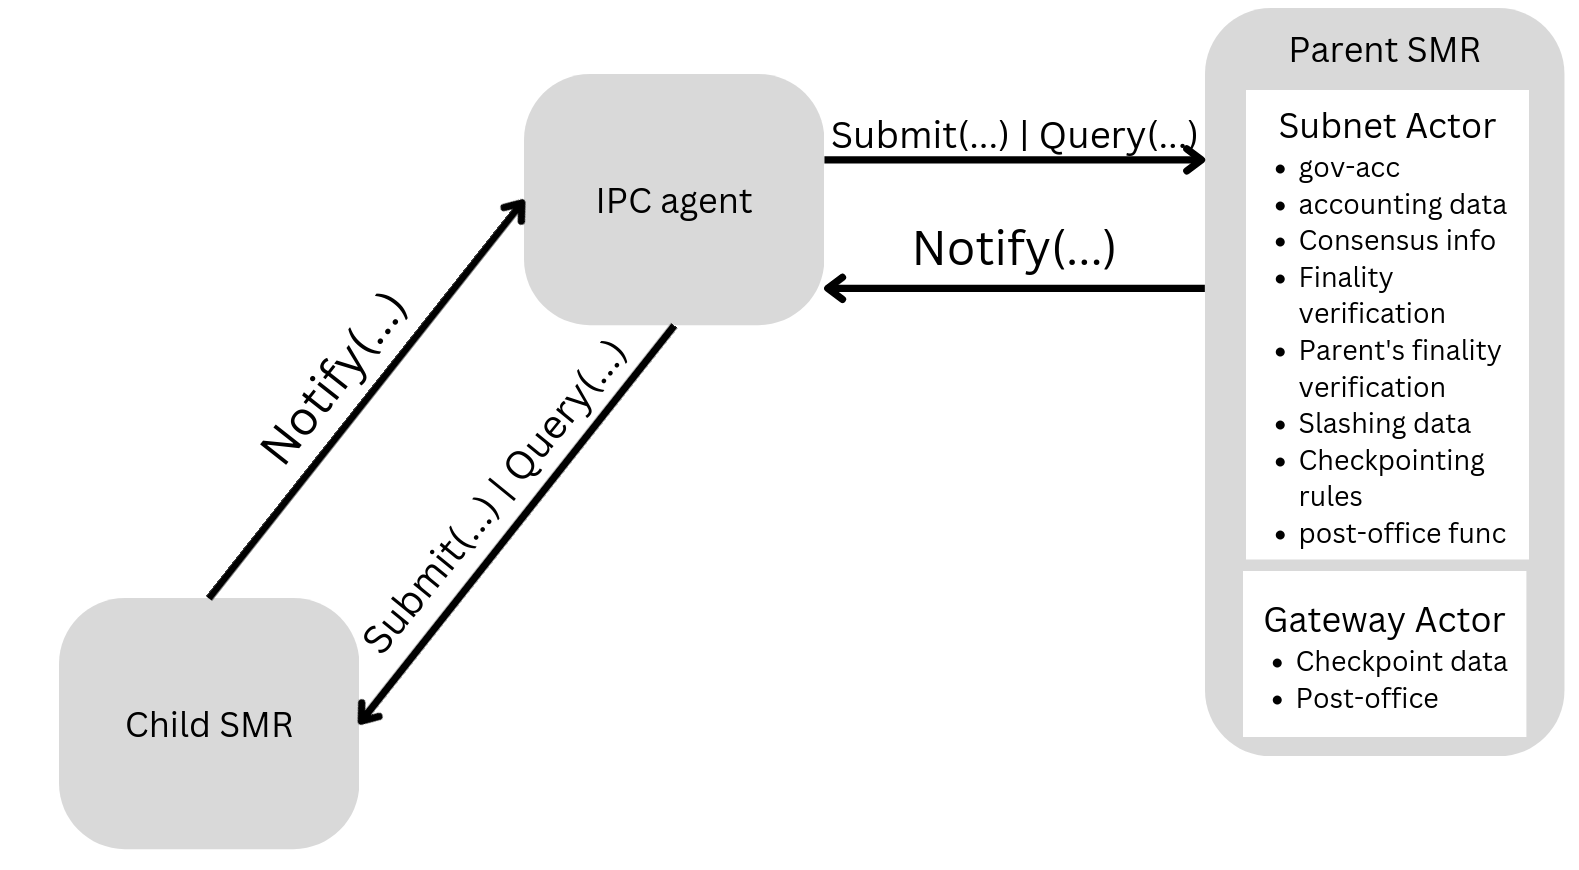
\includegraphics[width=0.75\textwidth]{compsintfs}
     \caption{The basic components and their interfaces.}
     \label{fig:interfaces}
 \end{figure}


\T{The state of \gw includes:}
\begin{itemize}
    \item Checkpoint data. The parent stores at the \gw each of the checkpoints from each direct child of it.
    \item Inter-subnet transactions service (denoted \postoffice). 
    \gw contains a registry of subnets and a functionality that can be used to transfer data from one subnet to another. 
    The \postoffice specifies the methods and the state locations that are used for these services.
    In particular, consider the following case involving a smart contract.%
    \footnote{When inter-subnet data transfer happens between users (Externally Owned Accounts --- \eoa --- in Ethereum's jargon), they can actively participate in the propagation via the \ipc agent that communicates with both the parent and child subnets. Smart contracts, on the other hand, do not have that power and, therefore, cannot communicate inter-subnets as efficiently as users (\eoa).}
    Smart contract $\textit{SmCt}$ emits an event~$e$ that contains $\textit{data}$ which is desired to reach the destination~\textit{dest} in a different subnet.
\end{itemize}
 
 
 
 % - IPC Functionality
 %  - Minimum required per subnet
 %    - Withdrawal/Deposits Interfaces
 %    - Other Operations? (Propagate?)
 %  - Enhancements
 %    - Checkpointing interfaces
 %    - Propagate
 %    - Reporting/Slashing interfaces
 %    - Atomic execution/swap, IBC-like bridges
 %  - Future stuff (google docs?)
 %    - Withdrawal at ancestor (skip parent(s)) (with timeout) etc.
\section{IPC functionality}
\label{sec:functionality}
We list in this section the functionality that should be provided by the IPC components. We first list the minimal functionality required for every subnet (deposits and withdrawals), to then extend it with enhanced functionalities. We model components as processes that produce and consume events. Events consumed by the IPC agent are the result of either a notification from one of the SMRs or the response of a query made by the IPC agent. Events produced by the IPC agent result in the IPC agent submitting a transaction that will change the state of the SMR that consumes the event.

We note that our focus is on the core functionalities, disregarding optimizations for the moment. Batching is a prime example of this. It is expected that batching will be a key optimization whenever \verifyGfinal{\tx}{\prf} is used, as calling \verifyGfinal{\tx}{\prf} can be costly. Batching allows us to perform multiple operations for one \verifyGfinal{\tx}{\prf} call, reducing its overall cost.

\subsection{Minimal Functionality}
\label{sec:minFunc}
We show in this section the functionalities for deposits and withdrawals.

\subsubsection{Deposits}
\label{sec:deposit}

\arp{Consider need to pause/remedy subnet after deposit (e.g. collateral not enough with new supply). IPC agent should check in that case}\\

A deposit is a transfer of funds (of some amount \fil) from user $\user_P$'s wallet in the parent subnet to user $u_C$'s wallet in the child subnet.
We assume that $u_P$ is a participant running a parent replica, a child replica, and an \ipc agent.%
\footnote{If $u_P$ does not run these processes, $u_P$ contacts a trusted participant that does and that performs the deposit on $u_P$'s behalf.}
The deposit is performed by the user controlling the \ipc agent as follows:
\begin{enumerate}
    \item The local \ipc agent submits to the parent \smr replica the corresponding (properly signed) transaction
    $\tx=\textit{Deposit}\left( \src, \fil, \sa.\textit{accounts}.\dest \right)$ with $\src=\user_P$ and $\dest = \user_C$.
    \item The parent SMR system orders and executes the Deposit transaction (provided $u_P$ has enough funds) by transferring $amt$ from $u_P$'s parent account to the \sa (concretely, to $u_P$'s account representation within the \sa). This effectively locks the funds within the \sa \dapp, until the \sa \dapp transfers it back to $u_P$'s account during withdrawal (see \Cref{sec:withdraw}).
    \item When the parent's replicated state that includes the transaction becomes final (for some SMR-system-specific definition of finality), the local parent replica notifies the local \ipc agent, potentially attaching a proof of finality of $PoF(tx)$ to the notification.%
    \footnote{The exact content of $PoF(tx)$ depends on the implementations of the SMR systems. It might contain, for example, a quorum of replica signatures, a Merkle proof of inclusion, or even be empty.}
    \item The \ipc agent constructs a transaction $\tx' = \textit{Deposited}\left(\langle  \src, \fil, \sa.\textit{accounts}.\dest \rangle, \prf \right)$ and submits it to the child SMR system.
    \item Upon ordering $tx'$, the replicated logic of the child SMR system mints \fil new coins and adds them to $\user_C$'s account.
\end{enumerate}

We show in \Cref{fig:deposit} the events being produced and consumed by the deposit functionality and in Algorithm~\ref{alg:deposit} the pseudocode per component to implement the functionality.

\begin{figure}[h]
     \centering
     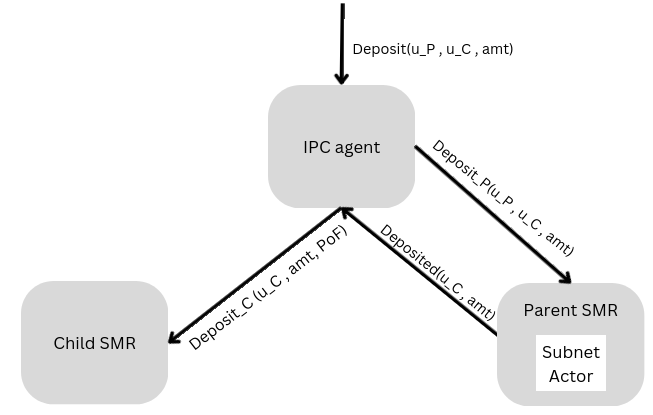
\includegraphics[width=\textwidth]{deposit}
     \caption{Events produced and consumed during a deposit.}
     \label{fig:deposit}
\end{figure}
 

\begin{algorithm}[H]
\footnotesize
\caption{Deposit operation}\label{alg:deposit}
  \DontPrintSemicolon
  \SetKwFunction{FMain}{Global}
  \SetKwProg{Pn}{Function}{:}{\KwRet}
  \SetKwInOut{Input}{input}
  \SetKwProg{Component}{$\blacktriangleright$ \bf}{:}{\KwRet}
  \SetKwFor{UponKW}{upon}{do}{fintq}
  \Input{\src account in parent, \dest account in child, amount~$\fil$}
   \Component{IPC agent}{
        submit $\tx=\textit{Deposit}\left( \src, \fil, \sa.\textit{accounts}.\dest \right)$ to parent \smr replica\;
  }
   %
   \Component{Parent \smr replica}{
   \UponKW{\tx}{
    move $\fil$ from \src to \sa.\textit{accounts}.\dest  \tcp*[r]{"lock" at parent}
    notify agent \texttt{ParentDeposited}(\tx)
   }
  }
  \Component{IPC agent}{
    \UponKW{notification of \texttt{ParentDeposited}(\tx) from parent \smr}{
        create \prf that \tx is final at parent \smr \tcp*[r]{see Sec.~? for details}
        submit \texttt{Deposited}$=\langle \tx, \prf \rangle$ to child \smr    
     }
  }
  \Component{Child \smr replica}{
    \UponKW{\texttt{Deposited}}{
        assert \prf for \tx\;
        increase \dest account by \fil
     }
  }
\end{algorithm}
One thing that differs a downward transaction (e.g., deposit) from an upward transaction (e.g., checkpoint) is that any participant that operates the child \smr replica also has visibility into the state of the parent \smr (albeit stale) through its local parent \smr replica. This enables the \textbf{local validity check} method to assert the finality at the parent (which may or may not be preferred over others).%
\footnote{\textbf{local validity check} (simpler, efficient, \textit{weaker guarantees}): $\prf$ contains a pointer to the block containing \tx  at the parent, together with the height~$h$ of that block.
 To assert that \tx is final, the child queries the parent about $TX$, if it exists -- return valid, else -- return invalid. If invalid but the parent is still below height~$h$, then query again when parent reaches height~$h$.
This is a test inside the child \smr process. Therefore, if we want this method (and I believe we do), we should widen the interface so that a child \smr can ask the agent to get data from the parent. However, this optimization comes at the expense of the encapsulation of components, that is, it entails tinkering with the child \smr code.}
            
\subsubsection{Withdrawals}
\label{sec:withdraw}

A withdrawal is a transfer of funds from user $u_C$'s wallet in the child subnet to some user $u_P$'s wallet in the parent subnet. We assume that $u_C$ is a participant running a parent replica, a child replica and an \ipc agent. The withdraw is performed as follows:
\begin{enumerate}
  \item $u_C$ triggers the $Withdraw(u_C, u_P, amt)$ event at the local \ipc agent.
    \item The local \ipc agent submits the corresponding (properly signed) transaction $tx = Withdraw_C(u_C, u_P, amt)$ to the child SMR system.
    \item The child SMR system orders and executes the Withdraw transaction, burning $amt$ funds in $u_C$'s account (provided $u_C$ has enough funds).
    \item When the child's replicated state that includes the transaction becomes final (for some SMR-system-specific definition of finality that has been defined in the SA), the local child replica notifies the local \ipc agent, potentially attaching a proof \prf that this state is final.%
    \item The \ipc agent constructs a transaction $tx' = Burned(u_P, amt, \prf)$ and submits it to the parent SMR system.
    \item Upon ordering $tx'$, the replicated logic of the parent SMR system updates the state of the SA transferring the funds from \sa (concretely, to $u_P$'s account representation within the \sa) to $u_P$'s account.
\end{enumerate}

 \begin{figure}[h]
     \centering
     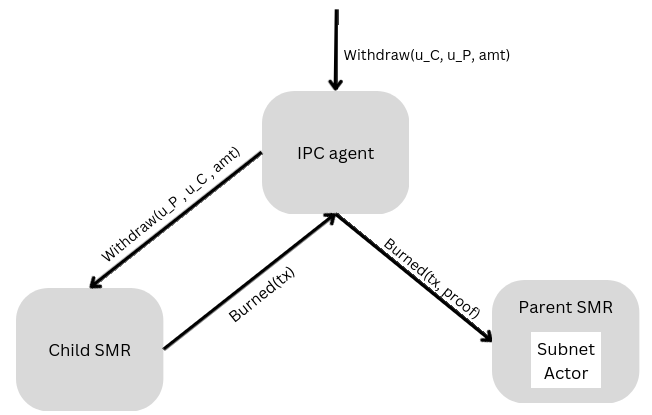
\includegraphics[width=\textwidth]{withdrawal}
     \caption{Events produced and consumed during a withdrawal.}
     \label{fig:withdrawal}
 \end{figure}
\begin{algorithm}[H]
\footnotesize
\caption{Withdraw operation}\label{alg:down}
  \DontPrintSemicolon
  \SetKwFunction{FMain}{Global}
  \SetKwProg{Pn}{Function}{:}{\KwRet}
  \SetKwInOut{Input}{input}
  \SetKwProg{Component}{$\blacktriangleright$ \bf}{:}{\KwRet}
  \SetKwFor{UponKW}{upon}{do}{fintq}
  % \Input{user~$\user$, amount~$\fil$, transaction \txnf}
   \Input{\src account in child, \dest account in parent, $\fil$ amount of coins}
   \Component{IPC agent}{
        submit $\tx=\textit{Withdraw}(\src, \fil, \dest)$ to child \smr\;
  }
   %
   \Component{Child \smr replica}{
   \UponKW{$\tx = \textit{Withdraw}(\src, \fil, \dest)$}{
    deduct $\fil$ from \src account at child \tcp{``burns" \fil in child}
    notify agent \texttt{Burned}(\tx)
   }
  }
  \Component{IPC agent}{
    \UponKW{notification of \texttt{Burned}(\tx) from child \smr replica}{
    
        create \prf that \tx is final at child \smr \tcp*[r]{see Sec.~? for details}
        submit $\tx'=\texttt{Burned}\left(\tx, \prf \right)$  to parent \smr replica
     }
  }
  \Component{parent \smr replica}{
    \UponKW{$\tx'=\texttt{Burned}\left(\tx, \prf \right)$}{
        assert \sa.\verifyGfinal{\prf}{\tx}\;
        move \fil coins from \sa.accounts[\src] to \dest
     }
  }
   
%    \Component{Child SMR}{
%    [\tx submitted by user, proposed, written]\\
%    \UponKW{\txnf written in Child SMR}{
%     decrease user fund's by $\fil$\\
%     Send \texttt{ChildWithdrawn(\tx, [$proof$])} to IPC agent \tcp*[r]{notify IPC agent}
%    }
%   }
%   \Component{IPC agent}{
%     \UponKW{\texttt{ChildWithdrawn(\tx, [$proof$])} notified by Child SMR}{
%     \If{$proof=$ \textbf{nil}}{
%          $proof \gets $\textit{generateProofOfGlobalFinality(\tx,...)} \tcp*[r]{Necessary steps for \tx to be ready to be submitted to Parent SMR}
%      }
%      \texttt{ChildWithdrawn(\tx, $proof$)} to parent SMR \tcp*[r]{Submit to parent}
%      }
%     \UponKW{\arp{State updated after Withdrawal}}{ \tcp*[r]{Notified when parents update state}
%       \arp{Check child subnet rules are still satisfied, remedy/close otherwise?}
%     }
%   }
%   \Component{Parent SMR}{
%   \UponKW{\texttt{ChildWithdrawn(\tx, $proof$)} submitted by IPC agent}{
%       \If{\sa.\verifyGfinal{\tx}{\prf}}{
%            [tx submitted by IPC agent, proposed, written]\\
%            \UponKW{\txnf written in Parent SMR}{
%                 reduce $\fil$ amount for user $\user$ in SA\\
%                 Parent SMR notifies IPC agent
%             }
%       }
%   }
% }
\end{algorithm}
\subsection{Enhanced Functionality}
\label{enhancedFunc}
\arp{From here below we need to add the gateway actor and refine the functionality, leave out till round of feedback for GW}
We show here a list of desirable functionalities that build upon the basic withdrawals and deposits.
\subsubsection{Checkpointing} A checkpoint contains a representation of the updated state of the child SMR system to be included in the parent SMR system. A checkpoint can be triggered by predefined events (i.e. periodically after a number of state updates, triggered by a specific user or set of users, etc.). As such, the checkpoint functionality may or may not be triggered by a user request on the child SMR. A checkpoint is performed as follows: 
\begin{enumerate}
\item If the predefined checkpoint trigger is met, then the IPC agent queries the child SMR replica for the updated state to be represented in this checkpoint.
\item The IPC agent creates a proof \prf that this updated state of the child SMR system is final, possibly compressing its representation of the state.
\item The IPC agent submits a transaction $\tx'=\texttt{Checkpoint}\left(\textit{state}, \prf \right)$ to the parent SMR replica
 \item Upon ordering $tx'$, the replicated logic of the parent SMR system updates the state of the SA according to the checkpoint state, if necessary.
\end{enumerate}

\begin{figure}[h]
     \centering
     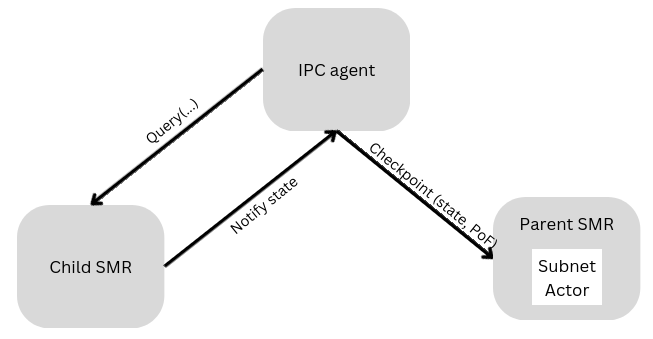
\includegraphics[width=\textwidth]{checkpoint.png}
     \caption{Events produced and consumed by the checkpointing functionality.}
     \label{fig:chkp}
 \end{figure}
\begin{algorithm}[H]
\footnotesize
\caption{Checkpoint operation}\label{alg:down}
  \DontPrintSemicolon
  \SetKwFunction{FMain}{Global}
  \SetKwProg{Pn}{Function}{:}{\KwRet}
  \SetKwInOut{Input}{input}
  \SetKwProg{Component}{$\blacktriangleright$ \bf}{:}{\KwRet}
  \SetKwFor{UponKW}{upon}{do}{fintq}
   \Component{IPC agent}{
        \If{trigger for checkpoint}{
            \textit{state} $\gets$ query the child \smr replica for the state\;
            create \prf that \textit{state} is final at child \tcp*[r]{Possibly compress \textit{state}}
        }
        submit $\tx'=\texttt{Checkpoint}\left(\textit{state}, \prf \right)$  to parent \smr replica
  }
  \Component{parent \smr replica}{
    \UponKW{$\tx'=\texttt{Checkpoint}\left(\textit{state}, \prf \right)$}{
        assert \sa.\verifyGfinal{\prf}{\textit{state}}\;
        $\sa.\textit{latestCheckpoint} \gets \textit{state}$
     }
  }
  
  % \Input{[User's checkpoint request]}
  % \Component{Child SMR}{
  %    \UponKW{State updated [ \textbar User's checkpoint request]}{ 
  %       [Write checkpoint request if any]\\
  %      Send \texttt{StateUpdated($st$)} to IPC agent \tcp*[r]{Notify IPC agent}
  %    }
  % }
  % \Component{IPC agent}{
  %   \UponKW{\texttt{StateUpdated($st$)} notified by child SMR}{
  %       \If{\texttt{SatisfiesCheckpointCondition($st$)}}{
  %          Create checkpoint \chkp\\
  %           $proof \gets $\textit{generateProofOfGlobalFinality($st$,...)} \tcp*[r]{Necessary steps for \tx to be ready to be submitted to Parent SMR}
  %           Submit \texttt{SubmitCheckpoint(\chkp)} to parent SMR
  %           }
  %       }
  % }
  % \Component{Parent SMR}{
  %     \UponKW{\texttt{SubmitCheckpoint(\chkp)} submitted by IPC agent}{
  %        [\chkp proposed, written]\\
  %        Refund fee to submitter \tcp*[r]{refund at parent for simplicity}
  %     }
  % }
\end{algorithm}

\subsubsection{Slashing} 
\guy{This section is immature for review (even a preliminary one)}\\
We show here the events produced and consumed by the slashing functionality. Given specific misbehavior from participants that is identified as Proofs of Fraud (PoFs), e.g.
gathering signed equivocating messages, the child SMR reports the PoFs to the IPC agent, which immediately forwards a slash a request to the parent SMR. \arp{Extend with need to verify if child SMR can continue, needs to remedy its depleted collateral or should be killed with latest checkpoint/state update}.
\begin{figure}[h]
     \centering
     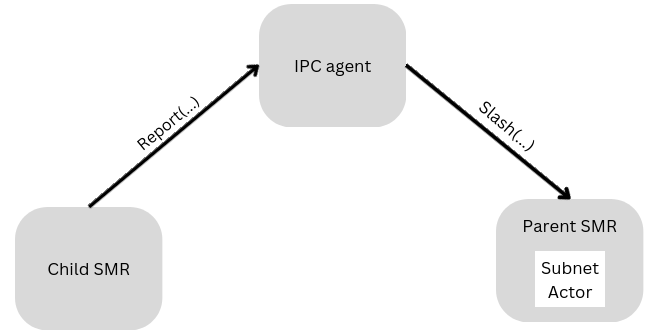
\includegraphics[width=\textwidth]{slash}
     \caption{Events produced and consumed by the slashing functionality.}
     \label{fig:report}
 \end{figure}\\

\begin{algorithm}[H]
\footnotesize
\caption{Slash Functionality}\label{alg:down}
  \DontPrintSemicolon
  \SetKwFunction{FMain}{Global}
  \SetKwProg{Pn}{Function}{:}{\KwRet}
  \SetKwInOut{Input}{input}
  \SetKwProg{Component}{$\blacktriangleright$ \bf}{:}{\KwRet}
  \SetKwFor{UponKW}{upon}{do}{fintq}
  \Input{-}
  \Component{Child SMR}{
     \UponKW{Proofs of fraud \pofs generated}{
       Notify \report to IPC agent
     }
  }
  \Component{IPC agent}{
    \UponKW{\report notified by child SMR}{
        Submit \slashop to parent SMR
    }
    \UponKW{\arp{State updated after slashing}}{
      \arp{Check child SMR rules are still satisfied, remedy/close otherwise?}
    }
  }
  \Component{Parent SMR}{
        \UponKW{\slashop submitted by IPC agent}{
         Update SA state slashing/excluding participants
         Notify SA update to IPC agent
        }
  }
\end{algorithm}


\subsubsection{\postoffice}
The \postoffice functionality is an inter-subnet transaction service. The main motivation for this functionality comes from a ``potential clients" request: enable a \dapp in one subnet to interact with a \dapp in a different subnet.\\
\guy{Edge case: a leaf subnet does not have a \sa and, therefore, no \postoffice. We can consider removing the \postoffice functionality from the \sa and to deploy it as an independent \dapp that will appear only once per subnet. In this case, it needs permissions to call \sa.\verifyGfinal{\tx}{\prf} function.}

\begin{algorithm}[H]
\footnotesize
\caption{\postoffice Functionality}\label{alg:po}
  \DontPrintSemicolon
  \SetKwFunction{FPropagate}{propagate}
  \SetKwProg{Pn}{Function}{:}{\KwRet}
  \SetKwInOut{Input}{input}
  \SetKwProg{Component}{$\blacktriangleright$ \bf}{:}{\KwRet}
  \SetKwProg{Empty}{\bf}{:}{\KwRet}
  \SetKwFor{UponKW}{upon}{do}{fintq}
  \Input{$\tx = \langle \data, \src, \dest, \prf \rangle$}
  \Component{\sa.\postoffice}{
     \UponKW{\postoffice.\propagate(\tx) }{
       \Case{\dest in current subnet}{
            \postoffice.\propagate\textit{HERE}(\tx)
       }
       \Case{\dest requires going up the tree}{
            \postoffice.\propagate\textit{UP}(\tx)
       }
       \Case{\dest requires going down the tree}{
            \postoffice.\propagate\textit{DOWN}(\tx)
       }
     }
     \UponKW{\postoffice.\propagate\textit{UP}(\tx) }{
       \If{\src not from this subnet}{
            assert(\sa.\verifyGfinal{\tx}{\prf})\;
       }
       \src.\textit{append(\sa's subnet id)}\;
       emit event \postoffice.UP$\langle \data, \src, \dest \rangle$
     }
     \tcp{\propagate\textit{DOWN}(\tx) is analogous to \propagate\textit{UP}(\tx)}
     \tcp{\propagate\textit{HERE}(\tx) is trivial}
  }
  \Component{parent \smr process}{
     \UponKW{event \postoffice.UP$\langle \data, \src, \dest \rangle$}{
        $\tx \gets \langle \data, \src, \dest \rangle$\;
        notify agent on \postoffice.UP(\tx)
     }
  }
  \Component{IPC agent}{
    \UponKW{notification of \propagate\textit{UP}(\tx) from child \smr}{
        create \prf that \textit{UP}(\tx) is final at child \smr\;
        $\tx_\textit{new}\gets\langle \textit{UP}(\tx), \prf \rangle$\;
        submit \sa.\postoffice.\propagate($\tx_\textit{new}$) to parent \smr
    }   
}
\end{algorithm}
\subsubsection{Atomic Execution}
TODO Discuss in Lanzarote?


\subsection{Future}
\label{sec:future}
 % - Implementations/templates
 %  - Different types and trade-offs of checkpoint triggers 
 %    - Periodically: time, #blocks, #withdrawn, etc.
 %    - At request: (this one is not governance funded)
 %    - Combinations of these 
 %    - Slashing functions
 %    - Atomic execution types?
 \section{An Instance of IPC}
 \label{sec:impl-tmpl}
 Here we describe the particular choices implemented by the Consensus Lab team.

The current implementation considers Filecoin as the root subnet\guy{I wrote it but I'm not sure this is the case...}, and Trantor as child subnets. For our interest it is important to note that Trantor is a BFT consensus protocol with immediate finality, and Filecoin is a longest chain style protocol with probabilistic finality. Therefore, as a \prf that a child subnet finalized a state we use a multisig on that state, the multisig must correspond to more than 2/3 of the child's validators voting rights as reflected by \sa at the time.%
\footnote{A next step in the implementation road-map is to offer a threshold signature mechanism instead of using a multisig. For now, multisigs serve the purpose of an MVP implementation.}
To verify the finality of a state at the parent, we use the fact that a participant has view in to a version of the parent blockchain (through its local parent replica process). In this case, \prf contains the block height~$h$ (and pointer to that block) at the parent subnet. A child replica then asserts with its parent that the state is final by checking with its local version of the parent blockchain at height~$h$. If the the local version at the parent replica did not reach height~$h$ yet, the child replica considers the state non-final/non-valid currently and checks again when the parent reaches height~$h$.
\section{Verifying the Finality of \tx{tx}}
\arp{I think this section should contain much more than this (but that perhaps this section does not follow our timelines for document completion (more of a complement of the document). Particular content here imo: Analysis for improvements wrt reference implementations (i.e. threshold signatures instead of everyone submitting checkpoints, governance account instead of no incentives, etc.); and Comprehensive list of different approaches for functionality/functions (like we had in the legacy document).}\guy{Agreed}
\label{sec:finality}
A main ingredient in any \ipcFull implementation is the creation and verification of a finality proof for a given \tx{tx} in some subnet. In the previous sections we left these functions opaque. For example, \sa.\verifyGfinal{\tx{tx}}{\prf} was used by the parent replica to verify the finality at the child subnet of \tx{tx}. The creation of \prf and the verification method at the child replica (for transactions of that occur at the parent subnet), are only hinted by plain text. There are multiple ways to implement these functionalities, each with its own trade-offs. Below we propose several such implementations.

 % - Components and their Interfaces
 %   - Parent subnet node
 %   - Child subnet node
 %   - IPC module
 %   - Subnet actor
 % - IPC Functionality
 %  - Minimum required per subnet
 %    - Withdrawal/Deposits Interfaces
 %    - Other Operations? (Propagate?)
 %  - Enhancements
 %    - Checkpointing interfaces
 %    - Propagate
 %    - Reporting/Slashing interfaces
 %    - Atomic execution/swap, IBC-like bridges
 %  - Future stuff (google docs?)
 %    - Withdrawal at ancestor (skip parent(s)) (with timeout) etc.
 % - Implementations/templates
 %  - Different types and trade-offs of checkpoint triggers 
 %    - Periodically: time, #blocks, #withdrawn, etc.
 %    - At request: (this one is not governance funded)
 %    - Combinations of these 
 %    - Slashing functions
 %    - Atomic execution types?
 
\newpage
\section{RAW LEGACY TEXT}
\textcolor{red}{Anything below should be ignored by readers}
\newpage
\section{TODO}
\begin{itemize}
    \item Collateral
    \item Schema
\end{itemize}
\section{Introduction}
\label{sec:intro}

Hierarchical Consensus is still an ongoing project, yet it already has an open source implementation available \cite{HCgit}.
The best architecture description available is~\cite{de2022hierarchical}.

This document will propose an architecture for the core functionality of \hc, on which additional layers/applications can be implemented.



The goal of \hc{} is to improve the scalability of blockchain systems.%
\footnote{This includes throughput increase as well as flexibility in Consensus mechanism choice.}
The chosen approach is by exploiting the ``locality'' phenomenon of users interactions.
In general, if users interact with each other in an arbitrary manner (or even uniformly at random), then there is no ``locality'' to exploit.
However, typically in practical systems, users tend to cluster in a way that users inside a cluster interact with each other more frequently than with outside users.
Roughly speaking, we wish to exploit this phenomenon by allowing a cluster to interact internally with less involvement of the main blockchain network.
Consequently, the internal interactions become cheaper and faster, thus, reducing the costs for the user. 
Moreover, the main blockchain also benefits from reduced load, since the demand to record every intra-cluster action is (partially) removed from the main blockchain.%
\footnote{Intra-cluster actions are summarized and recorded periodically to the main blockchain. So these interactions are not completely removed from the main blockchain, but the amount of resources that are demanded from the main blockchain significantly reduces.}


\section{Model}
\label{sec:model}

The vocabulary used throughout this document is summarized in the IPC Glossary \cite{glossary}.
The reader is encouraged to read the IPC Glossary before continuing.

\matej{When the Glossary becomes stable, we can maybe add it as an appendix to this document.}

\subsection{Computation and failure model}

We model \ipc as a distributed (``message-passing") system consisting of \emph{processes} that communicate by exchanging \emph{messages}%
\footnote{Network messages are not to be confused with Filecoin actor messages, that this document refers to as transactions.}
over a network. 
In practice, a process is a program running on a computer, having some state, and reacting to external events and messages received over a communication network.
We describe processes as exemplified in \Cref{alg:process-definition}.

\begin{algorithm}[H]
\footnotesize
\caption{Process definition.}\label{alg:process-definition}
  \DontPrintSemicolon
  \SetKwProg{Component}{$\blacktriangleright$ \bf}{:}{\KwRet}
  \SetKwFor{UponKW}{upon}{do}{fintq}
  \SetKw{Trigger}{trigger}
  variable = initial value\\
  variable = initial value\\
  ...\\
  \Component{process}{
     \UponKW{event(params...)}{
       \tcp{Logic to execute atomically}
     }
     \UponKW{message(params...)}{
       \tcp{Logic to execute atomically}
     }
     ...
}
\end{algorithm}

A process that performs all the steps exactly as prescribed by the protocols it is participating in is \emph{correct}.
A process that stops performing any steps (i.e., \emph{crashes}) or that deviates from the prescribed protocols in any way is \emph{faulty}.
If a process is correct or may only fail by crashing, it is \emph{benign}.
A non-benign process is \emph{malicious}.
\matej{We can remove terms we end up not using...}

In general, faulty processes can be malicious (Byzantine), i.e., we do not put any restrictions on their behavior, except being computationally bounded and thus not being able to subvert standard cryptographic primitives, such as forging signatures or inverting secure hash functions.
If the implementation of some component in our design requires additional assumptions on the behavior of faulty processes, they will be stated explicitly.
% We do not make a general statement about the fault tolerance of \ipc as a system, as to how many faulty processes the system can sustain.
% This depends on the final implementation of its components.

We use the term \emph{participant} to describe an entity participating in the system that controls one or more processes.
All processes controlled by one participant are assumed to be in the same trust domain -- they trust each other, i.e., assume each other's correctness.
For example, a participant in the child subnet will probably run multiple processes:
one for participating in the child subnet's protocol (child replica),
one for participating in the parent subnet (parent replica),
and one process that processes the information from the above two and submits transactions accordingly (\ipc agent).
We precisely define the replicas and the \ipc agent (all of them being processes) in \Cref{sec:components,sec:smr}.
The \ipc agent of a participant always assumes that the information it receives from "its own" child replica is correct.
However, messages received from another participant's replica or \ipc agent are seen as potentially malicious.

The synchrony assumptions may vary between different components of \ipc.
We thus state those assumptions whenever necessary, when describing concrete implementations of \ipc components.

\subsection{State machine replication (SMR) and \dapps}
\label{sec:smr}

\paragraph{SMR and replicated state.}
A \emph{state machine replication (SMR) system}%
\footnote{In this document, we use the terms ``SMR system" and ``blockchain" interchangeably.}
is a system consisting of processes called \emph{replicas}, each of which locally stores a copy of (or at least has access to) \emph{replicated state}
that it updates over time by applying a sequence of \emph{transactions} to it.
Without specifying the details of it, we assume that any process can \emph{submit} a transaction to an SMR system (we call such a process an \emph{SMR client})
and that this transaction will eventually be ordered and applied to the replicated state.
We call an SMR system that is part of \ipc a \emph{subnet}.

An SMR system guarantees to each correct replica that, after applying $n$ transactions to its local copy of the replicated state,
the latter will be identical to any other correct replica’s copy of the replicated state after applying $n$ transactions.
The replicas achieve this by executing an \emph{ordering protocol} to agree on a common sequence of transactions to apply to the replicated state.

Note that replicas do not necessarily all hold the same replicated state at any instant of real time,
since each replica might be processing transactions at a different time.
In this context, there is no such thing as “the current replicated state of the SMR system”.
There is only the current replicated state of a single replica.
The replicated state of the system is only an abstract, logical construct
useful for reasoning about transitions from one replicated state to another,
happening at individual replicas by applying transactions (at different real times).
When referring to a “current” replicated state, we mean the state resulting from the application of a certain number of transactions to the initial state.

\paragraph{Smart contracts.}
The replicated state of an SMR system can be logically subdivided into multiple \emph{\dapps} (a.k.a. actors in Filecoin).
A \dapp is a portion of the replicated state with well-defined semantics.
It defines the logic (e.g., expressed in a programming language, like Solidity in Ethereum)
that a replica needs to execute when applying transactions and the new state that results from it.

We model a \dapp as a logical object in the replicated state that contains arbitrary variables representing its state.
Its associated logic reacts to \emph{events} triggered by (1) the application of transactions or (2) execution of other (or even own) smart contract logic. We describe smart contracts as exemplified in \Cref{alg:dapp-definition}.

\begin{algorithm}[H]
\footnotesize
\caption{\dapp definition}\label{alg:dapp-definition}
  \DontPrintSemicolon
  \SetKwProg{Component}{$\blacktriangleright$ \bf}{:}{\KwRet}
  \SetKwFor{UponKW}{upon}{do}{fintq}
  \SetKw{Trigger}{trigger}
  variable = initial value\\
  variable = initial value\\
  ...\\
  \Component{\dapp name}{
     \UponKW{event(params...)}{
       \tcp{Logic to execute}
       \Trigger event(params...)
     }
     \UponKW{tx(params...)}{
       \tcp{Logic to execute}
       \Trigger event(params...)
     }
     ...
}
\end{algorithm}
Note that, despite using similar syntax to describe processes and \dapps, those are fundamentally different.
The former usually represent OS-level processes running on some physical machine,
the latter are an abstraction over the replicated state of an SMR system and their logic is being executed by all its replicas.
While a process can submit a transaction to an SMR system, a \dapp cannot.

\paragraph{Interaction between subnets.}
In \ipc, whole subnets need to interact, i.e., the replicated state of one subnet must react to (changes in) the replicated state of another subnet.
As the replicated state of every subnet is distributed among its replicas and evolves independently of other subnets,
we must establish a mechanism for interactions between the states of subnets.
In particular, we must explicitly link the two replicated states of two subnets.
More precisely, for any interaction between two subnets ($A$ and $B$), define block heights $h_A$ and $h_B$,
such that $A$'s replicated state at height $h_A$ considers $B$'s replicated state to have evolved exactly until $h_B$.

\paragraph{\PofsFull.}To this end, we define a \emph{\pofFull (\pof)} to be data that proves that an SMR system definitively reached a certain replicated state.
Regardless of the SMR system's ordering protocol's approach to finality (e.g., immediate finality for classic BFT protocols, or probabilistic finality in PoW-based systems),
a \pof convinces the the proof's verifier that the replicated state the \pof refers to will not be rolled back.
For example, for a BFT-based SMR system, a quorum of signatures produced by its replicas can constitute a \pof.
We denote by \emph{\pof(tx)} the proof that an SMR system reached a state in which transaction \emph{tx} already has been applied.



\subsection{Money}

For each pair of subnets in a parent-child relationship, we assume that there exists a notion of \emph{money} (measured in \emph{coins}) common to both subnets.%
\footnote{One can easily generalize the design to decouple the use of money between a parent and its child, but we stick with using the same kind of money in both subnets for simplicity.}
Each end user of the SMR system is assumed to have a personal wallet and a corresponding account in some subnet.

We also assume that the submission, ordering, and applications of transactions is associated with a monetary cost.
Each SMR client submitting a transaction to a subnet is assumed to have an account in that subnet, from which this cost is deducted.
If the funds are insufficient, the SMR system ignores the transaction.
\section{Skeleton}
\label{sec:Skeleton}

\begin{itemize}
    \item Every node in sub-net $\SN$ is also a node in all subnets that are ancestors of $\SN$. 
    This limits the practical depth of the hierarchy, since a ``deep'' node must divide its finite resources (bandwidth, computation, etc.) among all ancestor subnets. \guy{Should still offer great benefits. Should be analyzed theoretically under some assumption, for example: share of ``local'' interactions.}
    \begin{itemize}
        \item only consider full nodes; light nodes should be considered independently.
    \end{itemize}
    \item For each user there exists a hierarchy of accounts --- one for each sub-net it operates in. The account at $\SN$ contains the amount of tokens the user has at $\SN$ as well as the amount of tokens that are locked for use in the immediate children of $\SN$ (if the user has accounts there). 
    \begin{itemize}
        \item For simplicity, we consider a user always has its root account in the rootnet. In general, it is possible to have the root account at any subnet. However, once the root account is established the user can only open accounts in descendants of that subnet.%
        \footnote{To add accounts in other subnets, the user will need to create a new root account.}
    \end{itemize}
    \item An account interacts directly only with accounts at the same sub-net \textit{or} with the account's parent/children. \guy{My rational here is to provide the minimal necessary interface. See \cref{sec:inter subnet interactions} for details on inter sub-net interactions.}
    %transfers are made only between accounts at the same sub-net or between parent-child accounts of the same user.
    \begin{enumerate}
        \item \textbf{Intra sub-net interactions.} These interactions could include general operations (e.g., CAS) and are not restricted by \hc s design, they should follow the specific subnet definitions.
        \item \textbf{Parent--Child interactions.} These interactions are limited to token transfers between the user's parent/child accounts. \guy{Since both accounts are controlled by the same user, we do not need to worry about the flow of information between them --- it is the same entity and it knows what it's doing! We do need to reflect the state change to the entire system. That is, the new balances in the accounts (after tokens were transferred between the parent and child) must be visible to the respective sub-nets.}
    \end{enumerate}
    \item Interactions between parents and children are done periodically\arp{not necessarily} (e.g., together with checkpointing). \guy{clarify with Alfonso \cref{sec:P-C interactions}}
    \begin{itemize}
        \item This may be slower (in inter sub-net communication) but has the advantage of better isolation (and security) for sub-nets.
        \item A different option would be to allow parent-child interactions continuously in an atomic execution manner. However, this increases the complexity of the system and enables edge cases. For example, when executed alone, sub-net validators can easily ignore a user's attempt to transfer funds from its parent account. This censorship incurs a higher cost when it is tied to checkpointing the entire system.
    \end{itemize}
    \item Checkpointing is used for 2 purposes:
    \begin{enumerate}
        \item To enact the token transfers between parent-child accounts of the same user. E.g., releasing some of a user's tokens that are locked in $\SN$ to its account in \parent{$\SN$}. This is what enables the hierarchy to function. Necessary!\guy{also guarantees an account-grained firewall.}\arp{same as withdrawals}
        \item There is another use for checkpoints that is unnecessary for the \hc{} functionality but provides an additional benefit to the users. Periodically checkpointing the (complete) state of $\SN$ to its parent for added persistence that relies on the parent's guarantees. \arp{long-range attack mitigation}
        %\item to communicate changes upwards, i.e., releasing some of a user's tokens that are locked in $\SN$ to its account in \parent{$\SN$}.
    \end{enumerate}
    Notice that the two purposes of the checkpointing routine are theoretically independent of each other. In practice, however, they will probably be combined so further thought on the matter is warranted.
    \blue{Remark: while each sub-net can be a full SMR, for \hc s functionality, only accounting information (balance) needs to be communicated between child and parent sub-nets.}\arp{actually, only circulating supply suffices}
        \footnote{Simplifies things and should be sufficient. In order to reduce load from the parent, all of the changes that happened in the sub-net since the last checkpoint should be compressed into an efficient state-transfer operation. Hence, general state compression might be problematic. Accounts balance is easy to do and fits most uses. A future question would be extending to other states besides balances.}
    \item The creation and maintenance of a sub-net $\SN$ is governed by an \actor{} in \parent{$\SN$}.
    
\end{itemize}

\subsection{Checkpoint issues}
\red{TODO: explain compression issue.}\\
A checkpoint can be seen as a transaction in the parent net.\guy{Although crypto-econ lab approach is different, that is, they suggest special treatment for messages/actions that come from an \actor{} governing a subnet. I believe in a simpler design in which the aforementioned message is treated as any other message. I conjecture that this natural design (no need for special treatment) would be more robust in practice.}
However, several issues arise with regard to the cost of proposing a transaction.
A typical transaction is proposed by the user who wishes to get it into the blockchain, and hence, carries the associated costs --- specifically, the fee offered to the ``miners".
The proposing user, thus, decides solely on how much fee to offer. Simply putting, \emph{the one who receives the goods also pays for it}.
This forms the basis for classic economic theory of supply and demand.
On the other hand, in the case of the checkpoint fee, all nodes/users of $\SN$ decide on the fee and pay it (through the \actor), but not necessarily all of them have the same benefit from the checkpoint. 
For example, a user that did not perform any transactions since the last checkpoint might consider the checkpoint less urgent than a user that wishes to release funds to its parent account. 
\textbf{This issue requires further analysis!}\guy{To provide some default as a starting point, we can use a simple algorithm at the \actor{} that sets the proposed fee according to past information on the parent.}

\begin{itemize}
    \item If \parent{$\SN$} employs EIP1559, the problem is significantly mitigated. Setting the proposed fee based on an algorithm in the \actor{} is relatively safe since miners revenue is mostly block rewards and fees are expected to be negligible. Hence, miners have negligible incentive to discriminate transactions based on fees. (That is assuming that we trust EIP1559.)
    \item If \parent{$\SN$} employs the classic bidding mechanism to decide on which transactions to include in a block (i.e, highest fees win), the fact that the fee is payed from the ``common" account is problematic. It might incentive miners to manipulate the \actor 's fee-setting algorithm.
\end{itemize}

\subsection{Parent-Child Interactions}
\label{sec:P-C interactions}
\begin{itemize}
    \item currently parent-child communication is asymmetric. Parents send transactions down continuously but children send upwards only through checkpoints. This could be problematic (e.g., liveness of the protocol? Potential DDoS/flooding attack from the parent?). Suggestion: Initially, make transactions symmetric --- both directions happen through checkpoints.
    \begin{itemize}
        \item what is the subnet state included in the checkpoint that can be atomically modified with the top-down messages queued in the parent so the subnet knows the state from which to start again?
        \item how does a sub-net continues after a checkpoint? Is the checkpoint treated as a "genesis"?
        \item Can the sub-net continue optimistically? (probably, we can determine the delta and merge the ``extra operations" included in the parent).
    \end{itemize}
\end{itemize}

\subsection{Inter sub-net Interactions}
\label{sec:inter subnet interactions}
Conceptually, users are the ones that want to act, they do so by their accounts in the system.
If a user wishes to interact with an asset that is in the control of sub-net $\SN$ (e.g., a smart contract), she should open an account in that sub-net. \guy{Enabling an account from subnet $\SN_1$ to interact with resources in $\SN_2$ opens the door to long-term troubles.}

Fundamentally, cross-net messages are a chain of (upward) interactions between accounts of the same user until reaching a common ancestor with the target, then an interaction within this ancestor subnet, and finally a chain of (downward) interactions to the target recipient. Since both the upward and downward chains happen within the same user, it is her responsibility to make them happen (when your brain tells your hand to move, I don't need to interfere). The only interaction between distinct users happens in the same subnet and then we are in charge of making sure it happens properly.
Having said that, clearly, from a UX point of view, a gadget that helps the user execute the upward/downward chain of interactions will be important to users.
A service that streamlines the process of inter sub-net interactions (from a client's perspective) could be build on top of our system.
Nevertheless, in my opinion, cross-net messaging (with multiple hops) should not be a part of the core functionality but rather an add-on gadget. 


%%%%%%%%%%%%%%%%%%%%%%%%%%%%%%%%%%%%%%%%%%%%%%%
%%%%%%%%%%%%%%%%%%%%%%%%%%%%%%%%%%%%%%%%%%%%%%%

\section{Slashing}\label{sec:slashing}
Slashing is an additional functionality that aims at increasing the user's trust in a subnet.
In essence, by financially punishing misbehavior, participants are encouraged to follow the protocol.

Clearly, a general slashing mechanism that fits all possible subnets is impossible to devise. Hence, we suggest here a reference mechanism that fits several known Blockchain/SMR protocols~\cite{Filecoin,ETH,...}.

\subsection{Reference Slashing Mechanism}
We start by outlining the key principles:
\begin{itemize}
    \item The slashing is done at the parent. That means, the collateral of an $\SN$-validator is stored and managed at subnet $\parent{\SN}$.
    \item Slashing is done linearly with respect to the validator's voting power. E.g., if an equivocation from validator~$a$ with~$x_a$ of the voting power results in~$s_a$ deduction from $a$'s collateral, then an equivocation from validator~$b$ with $x_b=2x_a$ results in a deduction of $s_b=2s_a$ from~$b$'s collateral.
    \item Offences that are more of a ``malicious nature'' should incur higher penalties than ``benign'' offences.
\end{itemize}
Example of slashable offences:
\begin{enumerate}
    \item proposing equivocating blocks.
    \item voting on more than one block per epoch.
    \item proposing/voting on invalid block.
\end{enumerate}
\section{Miscellaneous}
\label{sec:misc}

\subsection{Shortcuts as a Service}
\red{Q: Can IBC be implemented independently as a ``shortcut" between subnets in the ``simple" model?}\\
A general IBC channel between subnets might be problematic since it would damage the subnet isolation guarantees. 
However, a service providing a ``shortcut" can be build as an application over the simple model, in a similar manner to bidirectional payment channels.
A service provider opens 2 accounts -- one in each subnet -- and deposits tokens in each. Denote these subnets by $\SN_A$ and $\SN_B$, and the service accounts as $s_A\in\SN_A$ and $s_B\in\SN_B$.
Now say that account $a$ from subnet~$A$ wants to transfer $m$~tokens to account $b\in\SN_B$. 
It can do so by transferring $m$ tokens in $\SN_A$ to $s_A$ and having $s_B$ transfer $m$ tokens in $\SN_B$ to $b$. Thereby creating a ``shortcut" instead of traversing the hierarchy tree.
Clearly, for this service~$a$ must pay fees to the service provider (to~$s_A$).

\arp{this is HTLCs}The trust/risk in this service falls only on the ones who participate in it, namely, the users behind~$a$ and~$b$, and the service provider.
Smart contracts can govern this service (instead of trusting the service provider).
Essentially, $a$ deposits the tokens in the smart contract which releases them to the control of $s_A$ given a proof that $b$ have received the tokens from~$s_B$.
The proof is based on $\SN_B$ guarantees, for example, the transaction appearing in $\SN_B$'s blockchain at a given depth.
The tokens would be released back to~$a$ in case a timer expired without~$s_A$ providing the proof.
To reduce costs in the common case, I suggest to include an ``cooparation'' release mechanism.
By adding the possibility for~$a$ to approve that the transaction happened to its satisfaction, the need to include a proof from~$\SN_B$ in~$\SN_A$'s blockchain is mitigated, when everyone is honest.
To encourage the use of the cooperation release by~$a$, the service provider can offer reduced fees whenever the release happens due to~$a$'a approval.

While this service entails liquidity costs (for the service provider), having it as an application on top of the HC framework provides several benefits.
(1) Service providers are expected to create shortcuts where they are most profitable, which should typically correlate with where they are most needed.
(2) Competition may arise among different service providers, driving for better service and reduced costs.
(3) All is done without central intervention.

% This service could easily be generalized to include multiple subnets. A service provider can have accounts in multiple subnets, thereby averaging the flow among many channels.

\newpage
\section{Pseudo-code}\label{sec:pseudocode}
In \cref{alg:join,alg:down,alg:up} we omit the fee paid by user~$\user$ to the governance account of subnet~$\SN_C$.
\begin{algorithm}[ht]
\caption{Join (very similar to move funds down)}\label{alg:join}
  \DontPrintSemicolon
  \SetKwFunction{FMain}{Global}
  \SetKwProg{Pn}{Function}{:}{\KwRet}
  \SetKwInOut{Input}{input}
  \SetKwFor{UponKW}{upon}{do}{fintq}
  \Input{user~$\user$, child subnet~$\SN_C$, parent subnet~$\PN_P$, amount~$\fil$}
    verify that $\user$ has an account in $\SN_P$ and that it has enough funds in $\SN_P$\;
    remove $\fil$ funds from $\user$'s account in $\SN_C$\;
    add  to the down-$\tx$-Batch the transaction: $\tx_\textit{create}(\user,\fil)$ instantiating an account for $\user$ with $\fil$ funds in $\SN_C$\;
    \UponKW{Propose down-$\tx$-Batch}{
        gov-account proposes down-$\tx$-Batch in $\SN_C$ with fee~$fee$ from $\SN_C$ governance account \tcp*[r]{this is an option for paying the fee.}
    }

    \UponKW{Execute down-$\tx$-Batch (in $\SN_P$)}{
        \For{each $\tx_\textit{create}$ in down-$\tx$-Batch}{
            $(\user,\fil)\gets \tx_\textit{create}$\;
            add account in $\SN_C.\textit{accounts}$ for user~$\user$
            add $\fil$ funds to $\user$'s account in $\SN_C$
        }
    } 
\end{algorithm}
%%=============================%%

%%=============================%%
\begin{algorithm}[ht]
\caption{Move funds down}\label{alg:down}
  \DontPrintSemicolon
  \SetKwFunction{FMain}{Global}
  \SetKwProg{Pn}{Function}{:}{\KwRet}
  \SetKwInOut{Input}{input}
  \SetKwFor{UponKW}{upon}{do}{fintq}
  \Input{user~$\user$, parent subnet~$\SN_P$, child subnet~$\SN_C$, amount~$\fil$}
  verify that $\user$ has accounts in both $\SN_P$ and $\SN_C$, and that it has enough funds in $\SN_P$\;
  remove $\fil$ fund from $\user$'s account in $\SN_P$\;
  add $\tx$ increasing $\user$'s account in $\SN_C$ by $\fil$ to the down-$\tx$-Batch\;
  
    \UponKW{Propose down-$\tx$-Batch}{
        gov-account proposes down-$\tx$-Batch in $\SN_C$ with fee~$fee$ from $\SN_C$ governance account \tcp*[r]{this is an option for paying the fee.}
    }

    \UponKW{Execute down-$\tx$-Batch (in $\SN_C$)}{
        \For{each $\tx$ in down-$\tx$-Batch}{
            $(\user,\fil)\gets \tx$\;
            add $\fil$ funds to $\user$'s account in $\SN_C$
        }
    }\tcp*[r]{If execution continuously fails (due to not enough fee) the money is lost.}

\end{algorithm}
%%=============================%%

%%=============================%%
\begin{algorithm}[ht]
\caption{Move funds up}\label{alg:up}
  \DontPrintSemicolon
  \SetKwFunction{FMain}{Global}
  \SetKwProg{Pn}{Function}{:}{\KwRet}
  \SetKwInOut{Input}{input}
  \SetKwFor{UponKW}{upon}{do}{fintq}
    \Input{user~$\user$, child subnet~$\SN_C$, parent subnet~$\SN_P$, amount~$\fil$}
  verify that $\user$ has accounts in both $\SN_C$ and $\SN_P$, and that it has enough funds in $\SN_C$\;
  remove $\fil$ funds from $\user$'s account in $\SN_C$\;
  add $\tx$ increasing $\user$'s account in $\SN_P$ by $\fil$ to the up-$\tx$-Batch\;
  
    \UponKW{Propose up-$\tx$-Batch}{
        gov-account proposes up-$\tx$-Batch in $\SN_P$ with fee~$fee$ from $\SN_C$ governance account \tcp*[r]{this is an option for paying the fee.}
    }

    \UponKW{Execute up-$\tx$-Batch (in $\SN_P$)}{
        \For{each $\tx$ in up-$\tx$-Batch}{
            $(\user,\fil)\gets \tx$\;
            add $\fil$ funds to $\user$'s account in $\SN_P$
        }
    }\tcp*[r]{If execution continuously fails (due to not enough fee) the money is lost.}
\end{algorithm}
%%=============================%%

%%=============================%%
\begin{algorithm}[ht]
\caption{Create Checkpoint}\label{alg:ckpt}
  \DontPrintSemicolon
  \SetKwFunction{FMain}{Global}
  \SetKwProg{Pn}{Function}{:}{\KwRet}
  \SetKwInOut{Input}{input}
  \SetKwFor{UponKW}{upon}{do}{fintq}
  
    \Input{\textit{prevCP}}
    \textit{newCP}$\gets$ get-snapshot($\SN_C$) \tcp*[r]{a recent state of $\SN_C$ individual accounts}
    verify-snapshot(\textit{newCP}) \tcp*[r]{E.g., a valid successor of \textit{prevCP} and signed by majority of validators.}
    \textit{diff}$\gets$ calculate diff from prevCP\;
    propose in $\SN_P$ to update \textit{prevCP} with \textit{diff} \tcp*[r]{fee should be paid from governance account}
    \For{each validator in $\SN_C$}{
        \UponKW{application of \textit{newCP} in $\SN_P$}{
            only offspring of \textit{newCP} will now be validated
        }
    }
\end{algorithm}
%%=============================%%

%%=============================%%
\begin{algorithm}[ht]
\caption{Default fee setting algorithm}\label{alg:fee}
  \DontPrintSemicolon
  \SetKwFunction{FMain}{Global}
  \SetKwProg{Pn}{Function}{:}{\KwRet}
  \SetKwInOut{Input}{input}
  \SetKwFor{UponKW}{upon}{do}{fintq}
  
to do...
\end{algorithm}
%%=============================%%

%%=============================%%
\begin{algorithm}[ht]
\caption{Example slashing mechanism (Depends on specific consensus mechanism)}\label{alg:slash}
  \DontPrintSemicolon
  \SetKwFunction{FMain}{Global}
  \SetKwProg{Pn}{Function}{:}{\KwRet}
  \SetKwInOut{Input}{input}
  \SetKwFor{UponKW}{upon}{do}{fintq}
    \Input{\textit{validator, proof}}  
    \If{\textit{proof} that \textit{validator} voted for more than 1 block in epoch}{
        slash \textit{validator} completely
    }
    \If{\textit{proof} that \textit{validator} proposed more than 1 block in epoch}{
        slash \textit{validator} completely
    }
    \If{\textit{proof} that \textit{validator} proposed more than 1 block in epoch}{
        slash \textit{validator} completely
    }
    \If{\textit{proof} that \textit{validator} proposed an invalid block}{
        slash \textit{validator} by a factor of $1/10$
    }

\end{algorithm}
%%=============================%%
\section{Notes form meeting at 2AUG22}
\label{sec:meetingNotes}
There are two different models to consider: (1) the ``IBC" model, and (2) the ``simple" model.

% IBC
In the IBC model \cite{IBC} (which might be the initial intention of \hc), accounts from different subnets can communicate with each other using bridges. This allows two accounts to perform cross subnet interactions directly using the 
IBC protocol, which in \hc s case will be the cross-net message transfer mechanism.\guy{I need to better understand \cite{IBC} to be sure, but it appears that interaction between two accounts from different subnets requires not only trust between the accounts but also that \emph{the two subnets trust each other}.}

% simple model
In the simple model (which is described in this document), accounts cannot communicate directly with other subnets, in general. Rather, their cross-net interactions are limited to basic operations between parent and child accounts. In particular, to token transfers between accounts of the same user. Moreover, in order for a user $u_i$ to interact with a user $u_j$ they must both have accounts on a shared subnet.\\

Besides the need for a more complex mechanism to support cross-net messages in the ``IBC" approach, the main difference comes from what is the offered tradeoff.
Essentially, in ``IBC", the scalability comes on the expense of trust, while in the ``simple" approach the scalability comes from locality, and is therefore limited by its existence.
In particular, IBC requires stronger trust assumptions (a user needs to trust all subnets in the path of a cross-net interaction), but does not need to maintain a hierarchy of accounts, while ``simple" only requires that a user trusts the common ancestor subnet, but also requires to have an account in the common ancestor.\\
%
\red{Q: How much benefits can be drawn from the ``simple" model (in terms of scalability)?}\\
\red{Q: How limiting is the stronger trust requirements on the usage of the IBC model?}\\
\red{Q: Can IBC be implemented independently as a ``shortcut" between subnets in the ``simple" model?}


\subsection{Additional points}
\begin{itemize}
    \item It might be that batching is the main benefit of implementing IBC via \hc. In that case, we should consider whether this can be treated orthogonally (e.g., via a dedicated smart contract), rather than entangling it with \hc. On the other hand, maybe the entanglement provides implementation benefits, e.g., speedup. \arp{probs in same smart contract but imo added feature: not necessary to spawn a subnet. 'Simple' -> base functionality, IBC -> optional added features}
    \item It appears that currently the system requires a single ``almighty" token to support the IBC implementation (which is sufficient for MVP). Using the simple approach, naturally supports internal token generation. The only requirement is that the balances of $\SN$ in \parent{$\SN$} are in a token that is supported in \parent{$\SN$}.
\end{itemize}

%%%%%%%%%%%%%%%%%%%%%%%%%%%%%%%%%%%%%%%%%%%%%%%%%%%%%%
%%%%%%%%%%%%%%%%%%%%%%%%%%%%%%%%%%%%%%%%%%%%%%%%%%%%%%
\section{Meeting Notes from Vaduz}

Money / coins / tokens can only be sent from a concrete account at the parent to a concrete account on the subnet

SA: Subnet actor (smart contract) on the parent, holding all information relevant for a single subnet.
$G$: Guy's account on the parent
$g$: Guy's account on the subnet
$g'$: Guy's subnet balance as seen by the parent, represented as an entry in the SA's account balances.

\paragraph{State of the smart contract contains:}
\begin{itemize}
    \item Account balances for all the children accounts in the subnet.
    \item A governance account and an associated policy how this account is funded and under which conditions money is transferred from it.
        The purpose of a governance account is to store funds associated with running the subnet (the subnet's "commons"). E.g., the transaction fees incurred by submitting checkpoints might be reimbursed from the governance account (under conditions specified by some policy). It can be funded, for example, by transaction fees within the subnet. The governance account might be involved in providing incentives for child validators to participate (rewards) and / or to behave correctly (slashing). The governance account has a corresponding account in the child subnet as well. It can be funded, e.g., through withdrawals from the child subnet.
    \item Validators' set + metadata (e.g. voting rights/collateral/stake/...)
    \begin{itemize}
        \item Consensus protocol
        \item Subnet configuration (probably a pointer to the data)
        \item Governance rules
    \end{itemize}
    \item A function $checkProofOfGlobalFinality(localState, proof)\rightarrow bool$. This function defines what constitutes a proof of global finality of a state of the child.
        E.g., this could be a set of signatures of subnet validators. For a longest-chain-based subnet, the definition of this function would involve a depth parameter, such that all blocks deeper than depth are considered final. If a reorganization of the child happens deeper than that depth, it can be considered as a failure of the whole subnet.
    \item Slashing functionality \arp{and checkpointing rules}
\end{itemize}

\paragraph{Interactions between parent and child}
It is likely that in practice, for efficiency reasons, multiple interactions will be batched together (possibly even combining withdrawals, deposits and checkpoint into a single transaction).
Nevertheless, we present here a cleaner version where operations are handled independently as it trivially generalizes to the batched version.
\begin{itemize}
    \item \textbf{DEPOSIT money (e.g. 2 coins) (transfer from G to g).}
    \begin{itemize}
        \item $\langle TX(G \rightarrow^{+2} SA:g')\rangle_{Guy}$: Transaction sending 2 coins from G to $SA:g'$, signed by Guy.
        \item Observer(s) of parent state create a TX for the child: $TX(g+2, proof)$ that adds 2 to g (when accepted as valid). The validity of this transaction must only depend on the transactions preceding it and itself.
        Example options for checking the validity of $TX(g+2, proof)$:
        \begin{enumerate}
            \item \textbf{on-chain voting}:
            When locally observing the parent state change, each subnet validator submits $\langle TX(g+2)\rangle_{Validator}$ to the child SMR system.
            When a quorum (e.g. $f+1$) such transactions signed by different validators are ordered, the last of them has the effect of increasing $g$ by 2.
            \item \textbf{off-chain voting}:
            Like on-chain voting, but all the transactions (signed by different validators) are gathered off-band and submitted (by any client to the child SMR system) as a single transaction $TX(g+2, proof)$, where the $proof$ consists of a quorum of child subnet validators' signatures.
            \item \textbf{local validity check} (simpler, efficient, \textit{weaker guarantees}): $proof$ contains a pointer to the block containing $\langle TX(G \rightarrow^{+2} SA:g')\rangle_{Guy}$ at the parent, together with the height~$h$ of that block.
            To validate the $TX$ the child queries the parent about $TX$, if it exists -- return valid, else -- return invalid. If invalid but the parent is still below height~$h$, then query again when parent reaches height~$h$.
            \item \textbf{subnet protocol integration}: Using PBFT as an example. Any client of the child subnet submits $TX(g+2)$ to the child (one is enough). On reception of a PBFT Preprepare message, a validator only sends the Prepare message once it observes the corresponding parent state change. This way, the child subnet's validators implicitly vote on the validity of $TX(g+2)$. Once it is committed, it is considered valid by all validators, even those that did not vote for it.
        \end{enumerate}
    \end{itemize}
    
    \item \textbf{WITHDRAW money (e.g. 2 coins) (transfer from g to G)}
    \begin{itemize}
        \item $\langle TX(g-2)\rangle_{Guy}$ (transaction ``burning" 2 coins from $g$, signed by Guy) on the child.
        \item Observer(s) of child state create a TX for the parent:  $\langle TX(SA:g' \rightarrow^{+2} G, proof)\rangle_{Guy}$ that decreases SA:g' by 2 and adds 2 to G (when accepted as valid). Validating this transaction must only depend on $proof$ and $SA$s internal state (which is visible at the parent).
        Example options for checking the validity of $\langle TX(SA:g' \rightarrow^{+2} G, proof)\rangle_{Guy}$:
        \begin{enumerate}
            \item \textbf{Threshold signature from the child subnet validators}:\footnote{An example is an $f+1$ threshold signature.}
            $proof$ contains a threshold signature from the child validators (which are listed in $SA$). A partial signature (for the threshold) from a validator~$v$ affirms that~$v$ considers $\langle TX(g-2)\rangle_{Guy}$ as stable in the child subnet.
            \item \textbf{Direct voting of the child validators:}\footnote{This is applicable very generally. However, it might be inefficient.}
            A quorum of the child validators submits a transaction (each validator a separate transaction) $\langle TX(SA:g' \rightarrow^{+2} G)\rangle_{Guy}$ to the parent. Only after enough (desired quorum size based on the validators is $SA$) such messages are appended to the parent ledger, the transaction $TX$ takes effect (transferring the money from $SA:g'$ to~$G$).
        \end{enumerate}
    \end{itemize}
    
    \item CHECKPOINT (include a representation of / reference to a particular version of the child's whole replicated state in the parent's replicated state) \guy{Think on who pays (and how) for $TX$ at the parent.}
    \begin{itemize}
        \item Observer(s) of child state identifies a condition for creating a checkpoint. Example for such conditions:
        \begin{enumerate}
            \item $\Delta$ blocks were appended to the child SMR since previous transaction,
            \item $\Delta$ money changed hands since previous checkpoint,
            \item enough fees were collected in a checkpoint request smart contract.
            \item Validator's will (most likely at its own expense, not that of the governance account). This could be a good approach where above conditions do not justify the overhead of periodic checkpoints (an instead this can  be left open to incentives)
        \end{enumerate}
        \item The observer then creates $\textit{data}$ and $\textit{proof}$ for the checkpoint, where $\textit{data}$ is the checkpoint data (or reference thereof) and $\textit{proof}$ is a proof of the validity of the data.
        Example options for $\textit{proof}$ and $\textit{data}$:
        \begin{enumerate}
            \item $\textit{data}$ is the diff between the state of the accounts in $SA$ (e.g.,~$SA:g'$) and the state of the accounts at the child SMR (e.g.~$g$). \ $\textit{proof}$ is a threshold signature from a quorum of the child subnet validators confirming $\textit{data}$ as well as the condition for creating a checkpoint. In addition, the $\textit{diff}$ might be required to sum to~0.
            \item \guy{provide additional example. ZK}
        \end{enumerate}
        \item The observer submits a checkpoint TX for the parent:  $\langle TX(\textit{data}, \textit{proof})\rangle_{Guy}$ that updates the state of $SA$ according to $\textit{data}$ if $TX$ is valid.
        Validating this transaction must only depend on $\textit{proof}$ and $SA$s internal state (which is visible at the parent).
        Note that the fee for TX is payed by G (the signer on TX), hence it should be reimbursed by $SA$s governance account upon the execution of TX.%
        \footnote{If there is a mechanism to directly charge SA:governance with the fee for a transaction signed by Guy, it would be better.}
        \item SA updates its state according to TX and might reimburse Guy for TX's fee from the governance account according to the SA's policy.
    \end{itemize}
    
    \item REPORT violation (for slashing purposes):
    The SA contains a \emph{slashing policy (sp)}. This policy defines
    \begin{enumerate}
        \item What constitutes a proof of misbehavior (PoM) ($sp.validate(PoM) -> bool$)
        \item The consequences of submitting a valid PoM ($sp.apply(PoM, metadata)$)
    \end{enumerate}
    Slashing works as follows:
    \begin{enumerate}
        \item Any user submits $\langle TX(PoM, metadata)\rangle$ to the parent. Metadata contains additional information about the TX, e.g., the identity of the submitting user.
        \item The execution of this transaction triggers a call to $SA.REPORT(PoM, metadata)$ (method of the SA).
        \item The implementation of the method invokes $sp.validate(PoM)$. The validity of the $PoM$ must only depend on the state of the SA and the $PoM$ itself.
        \item If the $PoM$ is valid, the SA invokes $sp.apply(PoM, metadata)$ that changes the internal state of SA and may produce additional internal transactions (applied directly to the state of the parent chain). For example, this might result in transferring part of the collateral of the offending child validator (identified through the $PoM$) that is locked in the SA to the governance account (or burning it), and/or transferring part of the validator's collateral to the user that submitted the PoM transaction (identified it the transaction's $metadata$).
    \end{enumerate}


    \item \textbf{POST-OFFICE for inter-subnet transactions:} $SA$ contains a functionality that can be used to transfer data from one subnet to another. In particular, consider the following case involving a smart contract (which, therefore, cannot be solved by deposit and withdraw operations).%
    \footnote{When the data transfers is between Externally Owned Users, it is typically better to use withdraw and deposit operations.}
    Smart contract $\textit{SmCt}$ emits an event~$e$ that contains $\textit{data}$ which is desired to reach the destination~\textit{dest}.
    \begin{enumerate}
        \item $\textit{SmCt}$ calls the functionality POST-OFFICE.\textit{propagate}$(\textit{data}, \textit{dest})$. According to \textit{dest}, this triggers a call to \pUp{}, \pDn{} or \pHr. (We leave out slight optimization for readability.)
        \setcounter{myCounter}{\value{enumi}}
    \end{enumerate}
    Below we describe only \pUp{} as \pDn{} can be deducted from it and \pHr{} is trivial.
    \begin{enumerate}
        \setcounter{enumi}{\value{myCounter}}
        \item The functionality \pUp{} handles a call $e$ only if one of the following holds:
        \begin{itemize}
            \item \textbf{A subnet-local call:} $\pUp(\textit{data}, \textit{dest})$ is called by a smart contract in the same subnet as \pUp. In that case, it emits an event $\textit{POST-OFFICE.propagateUp}=(\textit{src}=\textit{SmCt}, \textit{data}, \textit{dest})$ that will be propagated up.
            \item \textbf{A propagate from child call:} $\pUp(\textit{POST-OFFICE.propagateUp}, \textit{proof})$ is called, where $\textit{proof}$ validates that \textit{POST-OFFICE.propagateUp} was emitted in the child subnet (that is on the path to $\textit{propagateUp}.\textit{src}$) by the POST-OFFICE functionality in the child.
            Examples for $\textit{proof}$ are similar to those of WITHDRAW.
            In that case, \pUp{} emits an event $\textit{propagateUp}=(\textit{src}=\textit{SmCt}, \textit{data}, \textit{dest})$ that will be propagated up.
        \end{itemize}
        \item\label{step:obs} An observer of the child state submits a TX for the parent:  $\langle TX(\textit{propagateUp}, \textit{proof})\rangle_{Guy}$.
        Validating this transaction must only depend on $\textit{proof}$ and $SA$s internal state (which is visible at the parent).
        \item At the parent, once the proposal $\langle TX(\textit{propagateUp}, \textit{proof})\rangle_{Guy}$ is committed, it triggers \textit{POST-OFFICE.propagate} at the parent.
    \end{enumerate}
    Note that at step~\ref{step:obs} the EOA belonging to Guy pays the gas costs for TX.
    A mechanism for incentivizing Guy to propose TX is warranted. Purposely, we do not entangle the incentive with the propagate functionality, instead we allow for different incentive mechanisms to be used.
    Example for incentive mechanisms:
    \begin{itemize}
        \item \textbf{\textit{SmCt} is part of a smart contracts network:} This network (which has smart contracts covering the path) will reimburse Guy.
        \item \textbf{A third party service:} \textit{SmCt} pays a service that has an account in its subnet. This service has has proposers (or smart contracts to incentivize them) in every subnet on the path that will propose.
        \item \textbf{An interested EOA:} A user that is interested in the success of the transaction and has accounts covering the path proposes the propagating TXs and pays the fees.
        \item \textbf{POST-OFFICE as a third-party service:} Equivalently to a third-party service, the POST-OFFICE can provide proposing reimbursement services for entire network. We suggest to add this as an explicit opt-in option (not a default). Moreover, to reduce user disappointments and to encourage the deployment of advanced services, we suggest that the POST-OFFICE charges very conservatively (expensive prices) for the proposing incentivization service.
    \end{itemize}
    We stress that no incentive mechanism can guarantee that TX reaches from \textit{src} to \textit{dest}, since the required fees for the entire path are, in general, not known in advance.


    
      
    % \item \textbf{PROPAGATE-up data from a smart contract}\guy{This seems a bit tricky and needs to be thought of further, but I propose here an additional service for that purpose. \textbf{Need to think about gas fees!}}\\
    % Smart contract $\textit{SmCt}$ emits an event~$e$ that contains $\textit{data}$ which is desired reach the destination~\textit{dest} and needs to propagate up. For this we will have an additional functionality (or a specified new smart contract) which we call \pUp. %\textsc{PropUp}.
    % The functionality \pUp{} handles a call $e$ only if one of the following holds:
    % \begin{itemize}
    %     \item \textbf{A subnet-local call:} $\pUp(\textit{data}, \textit{dest})$ is called by a smart contract in the same subnet as \pUp. In that case, it emits an event $\textit{propagateUp}=(\textit{src}=\textit{SmCt}, \textit{data}, \textit{dest})$ that will be propagated up.
    %     \item \textbf{A propagate from child call:} $\pUp(\textit{propagateUp}, \textit{proof})$ is called, where $\textit{proof}$ validates that \textit{propagateUp} was emitted in the child subnet (that is on the path to $\textit{propagateUp}.\textit{src}$) by the \pUp{} functionality in the child.
    %     Examples for $\textit{proof}$ are similar to those of WITHDRAW.
    %     In that case, \pUp{} emits an event $\textit{propagateUp}=(\textit{src}=\textit{SmCt}, \textit{data}, \textit{dest})$ that will be propagated up.
    % \end{itemize}
    % \begin{enumerate}
    %     \item The smart contract $\textit{SmCt}$ calls \pUp$(\textit{data}, \textit{dest})$, where $\textit{dest}$ is the destination of the data. This happens on the child.
    %     \item On the child, \pUp{} emits an event $\textit{propagateUp}=(\textit{src}=\textit{SmCt}, \textit{data}, \textit{dest})$.
    %     \item An observer of the child state submits a TX for the parent:  $\langle TX(\textit{propagateUp}, \textit{proof})\rangle_{Guy}$.
    %     Validating this transaction must only depend on $\textit{proof}$ and $SA$s internal state (which is visible at the parent).
    %     Note that the fee for TX is payed by G (the signer on TX), we should think on a way to reimburse it.%
    %     \footnote{My initial thought is to add a list of payers along the path which will be in charge of proposing at their respected subnets.}
    %     \item At the parent, once the proposal $\langle TX(\textit{propagateUp}, \textit{proof})\rangle_{Guy}$ is committed, it triggers \pUp{} at the parent.
    % \end{enumerate}

    % \item \textbf{PROPAGATE-down data from a smart contract} works similarly to Propagate-up with the proofs resembling that of DEPOSIT rather than WITHDRAW. In addition, the functionality should be changed to PROPAGATE with UP or DOWN (or current subnet) being cases according to $\textit{dest}$.
\end{itemize}



\paragraph{Agreeing on parent state changes (e.g.)}

\subsection{Interface between software modules}
In addition to the smart contract~$SA$, we separate the software needed to run IPC into three abstract modules with defined interfaces:
\begin{itemize}
    \item \textbf{Parent validator:} The software that runs the parent blockchain. Note that in this module is also in charge of interacting with the IPC smart contract~$SA$, which is maintained at the parent subnet. Any update that the parent validator performs on the SA is notified to the IPC module.
    \item \textbf{Child validator:} The software that runs the child blockchain. Note that some of the rules the child blockchain must satisfy are listed in~$SA$. Any output operation (withdraw, checkpoint) is notified to the parent validator through the IPC module. 
    \item \textbf{IPC module:} The software that is in charge of the interactions between the two blockchains. This includes, for example, observers for the parent and child subnets. Note that this is not the a smart contract (it is not $SA$). It is a piece of software that runs at a node and mediates the interactions between the child and parent validator software. 
    
\end{itemize}
These three pieces of software interact through interfaces that consume and produce events.
\subsubsection{Deposits and Withdrawals}
 We show in Figures~\ref{fig:deposit-old} and~\ref{fig:withdrawal} the events that each interface consumes and produces during deposits and withdrawals, respectively. \\
Any other operation that augments withdrawals (e.g. checkpoints) is analogous to withdraw operations. Checkpoints may change in the payload being transferred, but require the same events to be committed/aborted.\\
We proceed to explain each event being consumed/produced at each module.
\begin{figure}
     \centering
     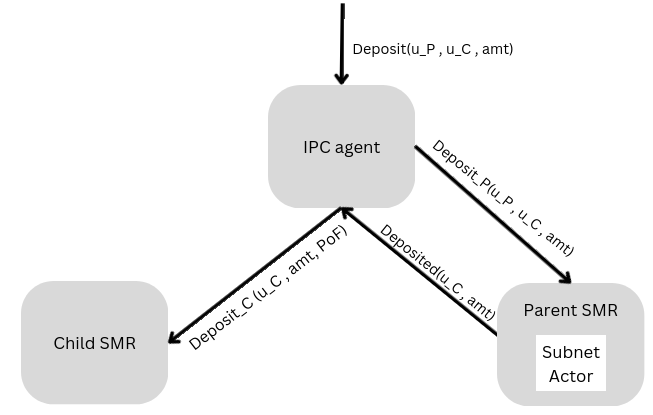
\includegraphics[width=\textwidth]{deposit}
     \caption{Events produced and consumed during a deposit.}
     \label{fig:deposit-old}
 \end{figure}
 
 \begin{figure}
     \centering
     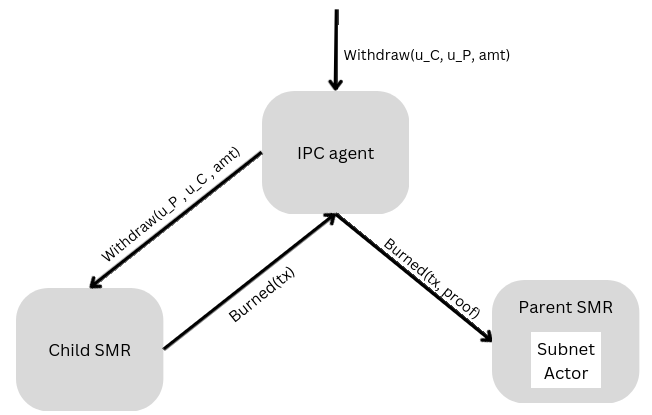
\includegraphics[width=\textwidth]{withdrawal}
     \caption{Events produced and consumed during a withdrawal.}
     \label{fig:withdrawal}
 \end{figure}
\noindent\textbf{Child Validator}\\
\textit{Deposits.} The child validator consumes an event \texttt{Deposited(TX)} produced by the IPC module upon which it updates its state in order to reflect this deposit. \\~\\
\textit{Withdrawals.} During operations that withdraw from child to parent subnets, the child validator first consumes a \texttt{WITHDRAW(TX)} from a user (or users) of the child subnet and then produces a \texttt{ChildWithdrawn(TX, [proof])} event to send to the IPC module. 
% The child validator does not yet terminate the withdrawal operation, as this may be aborted by the parent validator (if, for example, the withdrawal is invalid according to the state of the SA at the parent). The child validator eventually consumes a commit or an abort for each \texttt{ChildWithdrawn(TX, [proof])} that it produces. 
Depending on the type of subnet, the child validator can already provide a proof of global finality. If the child validator does not produce a proof of global finality then it is the job of the IPC module to produce such proof for the parent.\\~\\

\noindent\textbf{IPC Module}\\
\textit{Deposits.} The child validator first consumes a \texttt{ParentDeposited(TX)} transaction from the parent validator, and then performs the necessary operations to confirm the inclusion of the deposit into the child, depending on the type of deposit defined by the SA for this subnet and listed above in this document: on-chain voting, off-chain voting, local validity, etc. Once this deposit is confirmed by the IPC module, then the IPC module produces a \texttt{Deposited} event to be consumed by the child validator. The IPC module may also locally abort and not produce any events during deposits, should the deposit not be valid.\\~\\
\textit{Withdrawals.} During withdrawals, the IPC module first consumes a \texttt{ChildWithdrawn(TX, [proof])} event from the child validator, after which it produces a proof of the withdrawal that is valid for the SA at the parent (if the child subnet did not produce one already) and produces a \texttt{ChildWithdrawn(TX, proof)} to be consumed by the parent validator. 
% It is the responsibility of the IPC module to check the validity of the withdrawal given the state of the parent's SA, and to produce instead an \texttt{Abort} event to be consumed by the child validator if the SA's state is not consistent with the withdrawal. In the latter, it is possible that the IPC module finds proof of misbehaviour that should be reported, and in that case it also produces a \texttt{slash(...)} event to be consumed by parent, after which it will consume an event \texttt{Slashed(...)} from the parent validator and produce an event \texttt{Slashed(...)} to be consumed by the child validator.\\~\\
\noindent\textbf{Parent Validator}\\
\textit{Deposits.} The parent validator consumes a \texttt{Deposit(TX)} from a user (or users) and then produces a \texttt{ParentDeposited(TX)} event to be consumed by the IPC module.
\\~\\
\textit{Withdrawals.} During withdrawals, the Parent Validator consumes a \texttt{ChildWithdrawn(TX,proof)} event. 
% Then, it updates the current state of the SA, after which it produces a \texttt{Withdrawn(TX)} to be consumed by the IPC module. Alternatively, the parent might consume a \texttt{Slash(...)} event triggered by a withdrawal attempt, upon which it produces a \texttt{Slashed(...)}
\subsubsection{Other operations}
% \textit{Report/Slash.} There are two kinds of report operations: those that involve withdrawals, and those who are triggered at the child subnet but that should be reported at the parent. The former is already considered in the aforementioned flowchart for withdrawals, while the latter
We show reports in Figure~\ref{fig:report}. If the child validator detects provable misbehaviour, it notifies the IPC module through a \texttt{Report} event. Then, the IPC module follows the same path to request and notify slashing of the responsible deviants as the one showed for the withdrawal case.
\begin{figure}
     \centering
     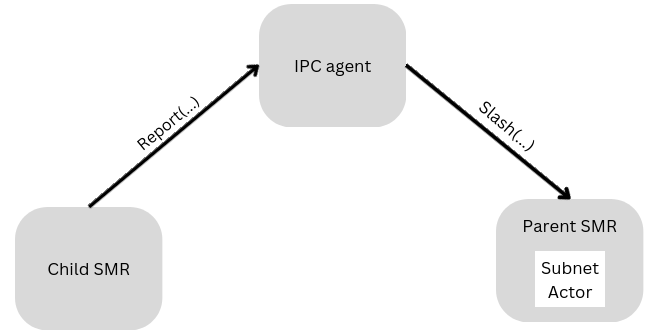
\includegraphics[width=\textwidth]{slash}
     \caption{Events produced and consumed during a report.}
     \label{fig:report}
 \end{figure}\\
 \textit{Checkpoints.} Checkpoints should follow the same procedure as withdrawals, except for: (i) the initial event that triggers the operation, as this is not necessarily a a transaction submitted by a user of the child subnet (most likely triggered by the IPC module); (ii) the payload of the events in the operation; and (iii) the local treatment of the events. The rationale for the events that are being triggered is analogous. 
 \arp{TODO: Propagate}
% \noindent \underline{IPC module interactions with the parent-validator:}%
% %\footnote{The interface is typically between two pieces of software on the same machine --- parent-node and child-node.}
% \begin{enumerate}
%     \item IPC-module queries the parent-validator if TX took effect in the parent (+ confidence parameter).
%     For example, the IPC-module observes (or is notified of) a relevant DEPOSIT transaction at the parent. 
%     \item IPC-module submits a transaction $TX$ to the parent-validator (the parent-SMR module). Examples:
%     \begin{itemize}
%         \item the IPC-module submits a WITHDRAW transaction $\langle TX(SA:g' \rightarrow^{+2} G, proof)\rangle_{Guy}$ to the parent-validator.
%         \item the IPC-module submits a CHECKPOINT transaction $\langle TX(SA:\textit{governance} \rightarrow^{+\textit{tip}} G, \textit{data}, \textit{proof})\rangle_{Guy}$ to the parent-validator.%
%         \footnote{Since~$G$ is the proposer and pays the transaction fee, the governance account ``reimburses"~$G$.}
%         \item the IPC-module submits a REPORT transaction to the parent-validator. \guy{TBD}
%     \end{itemize}
%     \item $getStateOf(SA)\rightarrow$ \guy{TBD}
    
% \end{enumerate}
% \vspace{2ex}

% \noindent \underline{Parent SMR invocations of $SA$ (the IPC smart contract):}
% \begin{enumerate}
%     \item \textbf{minimal interface} \texttt{DEPOSIT(subnet-account, amount)}\\
%     Example: \texttt{DEPOSIT($g'$, $2$)}\\
%     Increases a subnet client's balance by a given amount.
%     \item (\textbf{Including sanity check}) invoke DEPOSIT(Source, $SA:g$, amt). This enables the sanity check --- verify that Source (possibly restricted to $G$) has the funds to transfer.
%     \item \texttt{REPORT(violation, proof, reporter)} \guy{TBD}
%     \item apply \texttt{CHECKPOINT(data, proof)} \guy{TBD}\\
%     updates the data stored in $SA$ according to the new data in the checkpoint (e.g., updated account balances).
%     \item \texttt{Transfer(SA:governance$\rightarrow^{+\textit{amt}}G$, proof)} \guy{TBD}\\
%     Transfer money from the governance account to a specified account at the parent if $proof$ satisfy some condition. E.g., reimburse the proposer of a checkpoint.
% \end{enumerate}

% % \noindent \underline{IPC actor (smart contract) invocations of parent SMR:}
% % \begin{enumerate}
% %     \item \texttt{WITHDRAW(subnet-account, parent-account, amount)}\\
% %     Example: \texttt{WITHDRAW($SA:g'$, $G$, $2$)}\\
% %     Increases a parent client's balance by a given amount whilst reducing the child's account representation (the snapshot stored at SA in the parent) by the same amount.
% % \end{enumerate}

% \noindent \underline{IPC module interactions with the child-validator}

% \begin{enumerate}
%     \item $ProveGlobalFinality(tx) \rightarrow proof$: This function returns a proof that transaction $tx$ has been ordered and executed by the child SMR system and is final. This proof needs to be able to convince the SA (smart contract executed by the parent) of the $tx$'s finality. This is used for withdrawals: The SA only transfers the corresponding tokens to $G$ after verifying $proof$.
% \end{enumerate}

\subsection{additional points and future topics}
Non essential thing to think about in the future.
\begin{itemize}
    \item Entity observing parent replicated state and submitting corresponding transactions to the child SMR system (could be the user's laptop, a validator node, a third party, ...)
    \item finality function possibilities. E.g., varying according to amount, potentially slashed amount, network/faulty assumptions, etc. -> trade-off performance/security
    \item atomicity operations (atomic swap/atomic execution), IBC-like bridges 
    \item Alfonso: Fraud proofs and gas fees distribution. Two under-defined.
    \item Alfonso: if you don't mind including to your backlog of under-defined things: \url{https://github.com/consensus-shipyard/ipc-actors/issues/22} Also out of scope for M2, but really worth having for M3 and to answer future questions
\end{itemize}

 % - Intro
 %   - Overview
 % - Model
 % - Components and their Interfaces
 %   - Parent subnet node
 %   - Child subnet node
 %   - IPC module
 %   - Subnet actor
 % - IPC Functionality
 %  - Minimum required per subnet
 %    - Withdrawal/Deposits Interfaces
 %    - Other Operations? (Propagate?)
 %  - Enhancements
 %    - Checkpointing interfaces
 %    - Propagate
 %    - Reporting/Slashing interfaces
 %    - Atomic execution/swap, IBC-like bridges
 %  - Future stuff (google docs?)
 %    - Withdrawal at ancestor (skip parent(s)) (with timeout) etc.
 % - Implementations/templates
 %  - Different types and trade-offs of checkpoint triggers 
 %    - Periodically: time, #blocks, #withdrawn, etc.
 %    - At request: (this one is not governance funded)
 %    - Combinations of these 
 %    - Slashing functions
 %    - Atomic execution types?
 

% \section{Model}
\label{sec:model}

The vocabulary used throughout this document is summarized in the IPC Glossary \cite{glossary}.
The reader is encouraged to read the IPC Glossary before continuing.

\matej{When the Glossary becomes stable, we can maybe add it as an appendix to this document.}

\subsection{Computation and failure model}

We model \ipc as a distributed (``message-passing") system consisting of \emph{processes} that communicate by exchanging \emph{messages}%
\footnote{Network messages are not to be confused with Filecoin actor messages, that this document refers to as transactions.}
over a network. 
In practice, a process is a program running on a computer, having some state, and reacting to external events and messages received over a communication network.
We describe processes as exemplified in \Cref{alg:process-definition}.

\begin{algorithm}[H]
\footnotesize
\caption{Process definition.}\label{alg:process-definition}
  \DontPrintSemicolon
  \SetKwProg{Component}{$\blacktriangleright$ \bf}{:}{\KwRet}
  \SetKwFor{UponKW}{upon}{do}{fintq}
  \SetKw{Trigger}{trigger}
  variable = initial value\\
  variable = initial value\\
  ...\\
  \Component{process}{
     \UponKW{event(params...)}{
       \tcp{Logic to execute atomically}
     }
     \UponKW{message(params...)}{
       \tcp{Logic to execute atomically}
     }
     ...
}
\end{algorithm}

A process that performs all the steps exactly as prescribed by the protocols it is participating in is \emph{correct}.
A process that stops performing any steps (i.e., \emph{crashes}) or that deviates from the prescribed protocols in any way is \emph{faulty}.
If a process is correct or may only fail by crashing, it is \emph{benign}.
A non-benign process is \emph{malicious}.
\matej{We can remove terms we end up not using...}

In general, faulty processes can be malicious (Byzantine), i.e., we do not put any restrictions on their behavior, except being computationally bounded and thus not being able to subvert standard cryptographic primitives, such as forging signatures or inverting secure hash functions.
If the implementation of some component in our design requires additional assumptions on the behavior of faulty processes, they will be stated explicitly.
% We do not make a general statement about the fault tolerance of \ipc as a system, as to how many faulty processes the system can sustain.
% This depends on the final implementation of its components.

We use the term \emph{participant} to describe an entity participating in the system that controls one or more processes.
All processes controlled by one participant are assumed to be in the same trust domain -- they trust each other, i.e., assume each other's correctness.
For example, a participant in the child subnet will probably run multiple processes:
one for participating in the child subnet's protocol (child replica),
one for participating in the parent subnet (parent replica),
and one process that processes the information from the above two and submits transactions accordingly (\ipc agent).
We precisely define the replicas and the \ipc agent (all of them being processes) in \Cref{sec:components,sec:smr}.
The \ipc agent of a participant always assumes that the information it receives from "its own" child replica is correct.
However, messages received from another participant's replica or \ipc agent are seen as potentially malicious.

The synchrony assumptions may vary between different components of \ipc.
We thus state those assumptions whenever necessary, when describing concrete implementations of \ipc components.

\subsection{State machine replication (SMR) and \dapps}
\label{sec:smr}

\paragraph{SMR and replicated state.}
A \emph{state machine replication (SMR) system}%
\footnote{In this document, we use the terms ``SMR system" and ``blockchain" interchangeably.}
is a system consisting of processes called \emph{replicas}, each of which locally stores a copy of (or at least has access to) \emph{replicated state}
that it updates over time by applying a sequence of \emph{transactions} to it.
Without specifying the details of it, we assume that any process can \emph{submit} a transaction to an SMR system (we call such a process an \emph{SMR client})
and that this transaction will eventually be ordered and applied to the replicated state.
We call an SMR system that is part of \ipc a \emph{subnet}.

An SMR system guarantees to each correct replica that, after applying $n$ transactions to its local copy of the replicated state,
the latter will be identical to any other correct replica’s copy of the replicated state after applying $n$ transactions.
The replicas achieve this by executing an \emph{ordering protocol} to agree on a common sequence of transactions to apply to the replicated state.

Note that replicas do not necessarily all hold the same replicated state at any instant of real time,
since each replica might be processing transactions at a different time.
In this context, there is no such thing as “the current replicated state of the SMR system”.
There is only the current replicated state of a single replica.
The replicated state of the system is only an abstract, logical construct
useful for reasoning about transitions from one replicated state to another,
happening at individual replicas by applying transactions (at different real times).
When referring to a “current” replicated state, we mean the state resulting from the application of a certain number of transactions to the initial state.

\paragraph{Smart contracts.}
The replicated state of an SMR system can be logically subdivided into multiple \emph{\dapps} (a.k.a. actors in Filecoin).
A \dapp is a portion of the replicated state with well-defined semantics.
It defines the logic (e.g., expressed in a programming language, like Solidity in Ethereum)
that a replica needs to execute when applying transactions and the new state that results from it.

We model a \dapp as a logical object in the replicated state that contains arbitrary variables representing its state.
Its associated logic reacts to \emph{events} triggered by (1) the application of transactions or (2) execution of other (or even own) smart contract logic. We describe smart contracts as exemplified in \Cref{alg:dapp-definition}.

\begin{algorithm}[H]
\footnotesize
\caption{\dapp definition}\label{alg:dapp-definition}
  \DontPrintSemicolon
  \SetKwProg{Component}{$\blacktriangleright$ \bf}{:}{\KwRet}
  \SetKwFor{UponKW}{upon}{do}{fintq}
  \SetKw{Trigger}{trigger}
  variable = initial value\\
  variable = initial value\\
  ...\\
  \Component{\dapp name}{
     \UponKW{event(params...)}{
       \tcp{Logic to execute}
       \Trigger event(params...)
     }
     \UponKW{tx(params...)}{
       \tcp{Logic to execute}
       \Trigger event(params...)
     }
     ...
}
\end{algorithm}
Note that, despite using similar syntax to describe processes and \dapps, those are fundamentally different.
The former usually represent OS-level processes running on some physical machine,
the latter are an abstraction over the replicated state of an SMR system and their logic is being executed by all its replicas.
While a process can submit a transaction to an SMR system, a \dapp cannot.

\paragraph{Interaction between subnets.}
In \ipc, whole subnets need to interact, i.e., the replicated state of one subnet must react to (changes in) the replicated state of another subnet.
As the replicated state of every subnet is distributed among its replicas and evolves independently of other subnets,
we must establish a mechanism for interactions between the states of subnets.
In particular, we must explicitly link the two replicated states of two subnets.
More precisely, for any interaction between two subnets ($A$ and $B$), define block heights $h_A$ and $h_B$,
such that $A$'s replicated state at height $h_A$ considers $B$'s replicated state to have evolved exactly until $h_B$.

\paragraph{\PofsFull.}To this end, we define a \emph{\pofFull (\pof)} to be data that proves that an SMR system definitively reached a certain replicated state.
Regardless of the SMR system's ordering protocol's approach to finality (e.g., immediate finality for classic BFT protocols, or probabilistic finality in PoW-based systems),
a \pof convinces the the proof's verifier that the replicated state the \pof refers to will not be rolled back.
For example, for a BFT-based SMR system, a quorum of signatures produced by its replicas can constitute a \pof.
We denote by \emph{\pof(tx)} the proof that an SMR system reached a state in which transaction \emph{tx} already has been applied.



\subsection{Money}

For each pair of subnets in a parent-child relationship, we assume that there exists a notion of \emph{money} (measured in \emph{coins}) common to both subnets.%
\footnote{One can easily generalize the design to decouple the use of money between a parent and its child, but we stick with using the same kind of money in both subnets for simplicity.}
Each end user of the SMR system is assumed to have a personal wallet and a corresponding account in some subnet.

We also assume that the submission, ordering, and applications of transactions is associated with a monetary cost.
Each SMR client submitting a transaction to a subnet is assumed to have an account in that subnet, from which this cost is deducted.
If the funds are insufficient, the SMR system ignores the transaction.
% \input{sections/probabilisticInd.tex}
% \input{sections/lowerBound.tex}
% \input{sections/discussion.tex}
% ----------------------------------------------------------------
% ----------------------------------------------------------------

%%
%% The next two lines define the bibliography style to be used, and
%% the bibliography file.
\bibliographystyle{plain}
\bibliography{bibliography}

%%
%% If your work has an appendix, this is the place to put it.
\appendix
% ----------------------------------------------------------------
% ----------------------------------------------------------------
\newpage
% \section{Glossary}
\label{sec:gls}
\TODO{(Marko)Add IPC Glossary~\cite{glossary} here and move most of model down here}


% \input{sections/algorithm.tex}
% \input{sections/QvW.tex}
% \input{sections/Yao.tex}
% ----------------------------------------------------------------
% ----------------------------------------------------------------

%%%%%%%%%%%%%%%%%%%%%%%%%%%%%%%%%%%%%%%%%%%%%%%%%%%%%%%%%%%%%%%%%%
%%%%%%%%%%%%%%%%%%%%%%%%%%%%%%%%%%%%%%%%%%%%%%%%%%%%%%%%%%%%%%%%%%

\end{document}
\endinput
%%
%% End of file 